% Applied Intelligence manuscript. Original TMLR sources remain unchanged.
% Official Springer Nature December 2024 v3.1 class, numbered Basic style.
\documentclass[pdflatex,sn-basic,Numbered]{sn-jnl}
\usepackage{amsmath,amssymb,amsfonts,amsthm}
\usepackage{array,booktabs,multirow,graphicx,textcomp,xcolor,url}
\usepackage{placeins}
\hypersetup{hidelinks}
\makeatletter
\g@addto@macro\UrlBreaks{\do\-}
\makeatother
\graphicspath{{code/figures/}{figures/}}
\newtheorem{theorem}{Theorem}
\newtheorem{proposition}{Proposition}
\newtheorem{definition}{Definition}
\newtheorem{remark}{Remark}
\newtheorem{corollary}{Corollary}
\newtheorem{lemma}{Lemma}
\newtheorem{assumption}{Assumption}

\begin{document}
\title{From Graph Diagnostics to Model Decisions: Portfolio, Fallback, and Calibration}
\author*[1]{\fnm{Mengdan} \sur{Xue}}\email{17326961775@163.com}
\affil*[1]{\orgdiv{Faculty of Computational Mathematics and Cybernetics}, \orgname{Lomonosov Moscow State University}, \orgaddress{\city{Moscow}, \country{Russia}}}

\abstract{Graph diagnostics guide choices among trained models, so their utility depends on the candidate portfolio, calibration, and abstention fallback. We audit nine fixed graph-versus-multilayer-perceptron (MLP) policies on 11 node-classification datasets and ten seeds, measuring full-policy regret against the better validation-selected candidate. The frozen benchmark gives six graph architectures 24 tuning trials in total and MLP four trials. The historical Combined rule with MLP fallback incurs 7.46 percentage points of regret, compared with 0.26 for always-graph; four datasets contribute 95.1\% of its loss. Restricting the graph portfolio reverses some descriptive comparisons, with favorable frozen-record averages depending on Cornell and Wisconsin. Separate post-hoc retraining evaluates two input parameterizations and a 24-trial MLP search. Combined retains higher full-portfolio regret under MLP fallback, but a joint fallback/exclusion audit identifies local exceptions. Matching leave-one-dataset-out threshold calibration across ordinary homophily, adjusted homophily, and edge label informativeness preserves adjusted homophily's lower descriptive regret in all four input/budget configurations. With centered-scaled inputs and 24 MLP trials, it incurs 0.145 points against always-graph's 0.528: switching decisions yield 0.491 points of benefit and 0.108 of harm, with net gains confined to Cornell and Wisconsin. Primary dataset-level tests establish no superiority after multiplicity correction. The resulting offline audit connects scores to effective actions, reference headroom, and dataset-level losses, while distinguishing saved-score reconstruction from new training and independent validation.}
\keywords{Graph neural networks, Model selection, Graph diagnostics, Node classification, Benchmark evaluation, Decision regret}
\maketitle
\raggedbottom

\section{Introduction}

A graph diagnostic is useful for model selection if following its recommendation improves prediction. Its value depends on the candidate models, the score-to-action rule, and the fallback after abstention. A statistic that favors a graph convolutional network over an MLP may lead to different losses when the graph action selects among six trained architectures~\citep{kipf2017gcn,velivckovic2018gat,zhu2020beyond,lim2021linkx}.

Homophily research has developed class-conditional, feature, structural, and neighborhood-distribution statistics~\citep{luan2023whendo,platonov2023characterizing,zheng2024trihom,pmlr-v235-wang24u}. Learned selectors use graph characteristics and historical performance to choose models on new tasks~\citep{park2023metagl,park2023glemos}. We examine whether a diagnostic's advantage survives a change in candidate portfolio and which datasets determine the aggregate result. We then test whether calibration gains survive holding out related datasets together.

We audit graph-versus-multilayer-perceptron (MLP) decisions on 11 node-classification datasets and ten seeds. Validation selects candidates; oracle-portfolio regret measures the test accuracy lost by the final decision. Benefit and harm relative to always-graph identify useful and costly switches. A frozen nine-policy benchmark establishes the original case: a historical homophily rule with MLP fallback incurs 7.46 percentage points of regret against 0.26 for always-graph. Primary dataset-level tests establish no superiority after multiplicity correction. Separate post-hoc retraining and diagnostic analyses test the boundaries of that result.

A training-label-only Gaussian Naive Bayes adaptation of the Classifier-based Performance Metric (CPM) improves on both constant choices in all 12 restricted GCN/GAT configurations. It loses to always-graph in the four full-portfolio configurations. Roman-empire contributes 78.7--86.5\% of that loss; omitting it reverses three comparisons. Adjusted homophily has lower full-portfolio regret under leave-one-dataset-out (LODO) calibration, but its gains vanish or reverse under source-group holdout. Jointly withholding Cornell and Wisconsin produces an always-graph rule for both datasets in every full-portfolio configuration. Table~\ref{tab:contribution_map} gives the comparisons for one input/budget setting; subsequent sections report all configurations.

\begin{table}[tbp]
\centering
\caption{Connected decision comparisons under CS inputs and 24 MLP trials. Regrets are descriptive percentage points. The graph reference and oracle are recomputed for each portfolio and dataset set. The full 11-dataset set remains primary.}
\label{tab:contribution_map}
\small
\setlength{\tabcolsep}{3pt}
\begin{tabular}{@{}llrr@{}}
\toprule
Decision setting & Selector & Regret & Always-graph \\
\midrule
GCN, all datasets & CPM-.5 & 0.172 & 7.468 \\
Full portfolio, all datasets & CPM-.5 & 1.561 & 0.528 \\
Full, omit Roman-empire & CPM-.5 & 0.232 & 0.580 \\
Full, all datasets & Adjusted homophily, LODO & 0.145 & 0.528 \\
Full, all datasets & Adjusted, source-group holdout & 2.538 & 0.528 \\
\bottomrule
\end{tabular}
\end{table}

The audit extends CPM's paired-classifier evaluation to portfolio decisions and tests adjusted homophily and label informativeness as selection inputs. It complements GLEMOS's learned selection setting by tracing individual switches and their dependence on calibration sources. Released code reconstructs policies from retained candidate records and regenerates bound inputs from public data. The appendices provide mechanistic context through an auxiliary Gaussian calculation and graph intervention.

\section{Related work}
\label{sec:related}



\subsection{Graph statistics and model performance}

Edge homophily summarizes whether adjacent nodes share labels, but a global fraction omits class imbalance, feature geometry, neighborhood distributions, and local variation~\citep{mcpherson2001homophily,zhu2020beyond,ma2021homophily}. Post-aggregation similarity, adjusted homophily, label informativeness, and local characterizations describe additional aspects of message-passing behavior~\citep{luan2022linkx,platonov2023characterizing,loveland2024local}.

Several diagnostics address relative model performance directly. \citet{luan2023whendo} analyze node distinguishability and introduce the Classifier-based Performance Metric (CPM). \citet{zheng2024trihom} disentangle label, structural, and feature homophily; their 31-dataset study compares Tri-Hom with 17 metrics, including correlations with GCN-, GraphSAGE-, and GAT-versus-MLP gaps. Under a heterophilous stochastic block model, \citet{pmlr-v235-wang24u} relate separability gain to neighborhood-distribution distance and degree. These approaches characterize richer signals than the simple threshold rules used in our primary case studies. The post-hoc CPM-GNB adaptation in Section~\ref{sec:cpm_results} tests one such feature-based signal under the same decision audit.

Benchmark protocols affect the interpretation of these comparisons. Repeated splits and standardized graph collections expose sensitivity to splitting, tuning, and dataset selection~\citep{shchur2018pitfalls,hu2020ogb}. Reassessments of heterophilous benchmarks and homophily metrics further emphasize protocol quality~\citep{platonov2023heterophilous,luan2024reevaluating}. Dataset-level inference distinguishes variation across tasks from repeated seeds on the same task~\citep{demsar2006statistical}. We use paired evaluation and restrict label-dependent diagnostics to training labels. Recent preprint work also examines homophily-aware split construction to control relational composition across folds~\citep{jami2026stratification}. Our comparisons use the retained splits; sensitivity to alternative split designs remains untested.

\subsection{Architectures and the candidate portfolio}

Graph architectures differ in the signals they propagate and combine. H2GCN separates ego and neighbor representations and uses two-hop neighborhoods~\citep{zhu2020beyond}; LINKX separates structural and feature processing~\citep{lim2021linkx}; GPR-GNN learns a combination of propagation depths~\citep{chien2021gprgnn}. A recent preprint uses final-layer and head refitting to separate recoverable information from classification failure~\citep{ness2026rarity}. This distinction reinforces the need to audit the trained baseline before attributing a model gap to graph structure. Training depth, regularization, and representation contraction also affect predictive performance~\citep{oono2020exponential,chen2020measuring,rong2020dropedge,zhao2020pairnorm}. A one-hop mixing statistic therefore faces a different prediction problem when the graph action selects among these trained candidates. We examine that dependence using GCN, GAT, GraphSAGE, H2GCN, LINKX, and GPR-GNN, then restrict the portfolio while holding the diagnostic decisions fixed.

\subsection{Model selection and graph-signal controls}

Graph model selection already includes architecture search and learned selection across tasks. Auto-GNN searches architectures for a graph task~\citep{zhou2020autognn}. MetaGL selects graph-learning models using meta-graph features and historical performance~\citep{park2023metagl}; GLEMOS benchmarks instantaneous selection across 366 models and 457 graphs~\citep{park2023glemos}.

Using a published statistic for model selection requires specifying its label access, graph operator, input map, and score-to-action rule. A correlation study alone does not specify these choices.

These approaches predict different outcomes. CPM uses feature-based hypothesis tests to indicate the advantage of a graph-aware model over its paired graph-agnostic model~\citep{luan2023whendo}. Tri-Hom combines label, structural, and feature information; its evaluation measures correlations with model performance and graph--MLP gaps~\citep{zheng2024trihom}. GLEMOS selects models on unseen graphs from historical performance records and graph features, before fitting candidates on those graphs. It evaluates selection and ranking quality across transfer settings~\citep{park2023glemos}. We examine full-policy accuracy loss, abstention fallback, and available improvement as the candidate portfolio changes. Fixed threshold policies allow each decision to be traced, although they are not representative of all published diagnostics. The analysis uses established evaluation principles to locate policy losses and reversals in relative performance.

Our target is a binary graph-portfolio-versus-MLP action evaluated through oracle-portfolio regret and abstention coverage. The reference policies are always-graph, always-MLP, random, and direct validation selection. Each architecture receives four trials, yielding unequal aggregate search budgets for the six-architecture graph action and the single-architecture MLP action. This resource asymmetry is part of the evaluated decision problem.

Strong feature-only baselines and edge controls help interpret that decision. Well-tuned MLPs can be competitive when node features encode graph information~\citep{katsman2026necessary}, while edge-removal controls show that models can exploit graph structure even when it hurts generalization~\citep{bechler2024graphs}. Our degree-preserving rewiring intervention provides complementary evidence about graph signal. It changes class mixing and higher-order organization together, so it does not isolate homophily. Its role is to assess structural signal separately from the utility of the diagnostic policies.

The fixed-degree Gaussian calculation in Appendix~\ref{sec:snr} describes how correlation, degree, and feature strength interact under a prescribed linear average. Contextual stochastic-block-model recovery theory and finite-depth embedding analyses provide related theoretical perspectives~\citep{lu2023contextual,pmlr-v269-dalle25a}. The calculation describes aggregation moments; the recorded policy comparisons measure decision utility within the evaluated configurations.

\section{Decision-evaluation protocol}
\label{sec:protocol}

\subsection{Graph-versus-MLP decision}

The unit of evaluation is a dataset--seed pair $u$. Within each unit, validation performance selects one feature-only MLP and one graph model from GCN, GAT, GraphSAGE, H2GCN, LINKX, and GPR-GNN. Every architecture receives the same four-trial tuning budget, and exact validation ties are broken by model identifier. Let $a_u^{\mathrm{M}}$ and $a_u^{\mathrm{G}}$ denote the held-out test accuracies of the selected MLP and graph model. The evaluator reads each selected test result once; no diagnostic can affect training or hyperparameter selection. The resulting actions are portfolios: graph is the validation-selected member of six architectures, whereas MLP is the validation-selected configuration of one architecture.

We use a frozen practical margin $\delta=0.01$ to define the target action:
\begin{equation}
y_u =
\begin{cases}
\mathrm{G}, & a_u^{\mathrm{G}}-a_u^{\mathrm{M}}>\delta,\\
\mathrm{M}, & a_u^{\mathrm{G}}-a_u^{\mathrm{M}}\leq\delta.
\end{cases}
\label{eq:decision_target}
\end{equation}
Every rule uses this asymmetric target: graph must exceed MLP by more than one percentage point, and ties favor MLP.

\subsection{Per-architecture training and selection}

Table~\ref{tab:frozen_training} records the training grid. Each PyTorch trial~\citep{paszke2019pytorch} minimizes cross-entropy with Adam and retains the checkpoint with highest validation accuracy, then lowest validation loss and earliest epoch. Training stops after 100 stale epochs or 500 epochs in total. The grid crosses learning rates $\{0.01,0.005\}$ and dropout rates $\{0.5,0.7\}$, with width 64 and weight decay $5\times10^{-4}$. Each architecture independently selects one of its four trials and evaluates the chosen checkpoint once on the held-out test set. The six-architecture graph portfolio therefore searches 24 trial configurations, compared with four for MLP.



The split targets 60/20/20 for train/validation/test and is regenerated deterministically for seeds 0--9. Each class must contain at least three nodes, with at least one assigned to each of the training, validation, and test sets. Integer per-class floors make the realized proportions approximate, especially for small WebKB graphs; the actual counts are reported in the reproducibility summary. Every unit stores the source commit, canonical configuration digest, processed-data checksums, split identifier, four trial records, selected checkpoint, and environment provenance. The v1 and v2 JSON specifications differ only in the pre-outcome eligibility amendment described in Section~\ref{sec:prospective}; the later Squirrel amendment changes only the execution timeout.

The frozen protocol in this section governs the original benchmark. Subsequent portfolio analyses are post-hoc, and the additional preprocessing and training diagnostics use separately recorded configurations and information boundaries. Their status and scope are identified where they are reported.

\subsection{Decision-time information and policies}

Full node features and graph structure are available because they are model inputs. Label-dependent statistics use the subgraph induced by training nodes. Edge homophily $h_1$ is the label-agreement fraction on its edges. For the two-hop statistic $h_2$, a center with training-subgraph degree $d_T$ is sampled with probability proportional to $d_T(d_T-1)$, then two distinct neighbors are sampled uniformly without replacement. All three nodes therefore belong to the training set. The estimate is the mean endpoint-label agreement over 50,000 sampled ordered length-two paths, using the split seed plus 200,000 as the NumPy generator seed. Paths may repeat across draws, and adjacent endpoints are included when they form a length-two path; this is a path-weighted statistic, not strict distance-two homophily. If no eligible edge or path exists, the corresponding statistic is missing. Test labels, test accuracy, and statistics computed from test labels are forbidden diagnostic inputs; the evaluator rejects records that violate this boundary.

This is an offline audit of predictive decision utility: all candidate models are trained to supply common outcomes, and regret measures the test accuracy lost by selecting among them. Table~\ref{tab:diagnostic_policies} distinguishes each policy's required information and decision stage. An early family choice still requires fitting and selecting a model within that family. Validation selection provides a reference for decisions made after both families have been tuned. The evaluation measures accuracy loss and coverage; training-cost savings and deployment efficiency are outside its measured outcomes.

Table~\ref{tab:diagnostic_policies} lists the nine policies. The Combined rule has an exploratory origin: its exact $0.55/0.40$ thresholds were fixed in the specification and scorer on 8 August 2026, after inspection of legacy aggregates and before generation of the primary records. The final 110 units were not used to adjust them. Appendix~\ref{app:execution_details} retains the threshold provenance; the scope is a pre-specified primary analysis rather than whole-project preregistration. The policy chooses graph when training-only edge homophily is at least $0.55$; below that threshold, it chooses MLP when MLP validation accuracy is at least $0.40$ and otherwise abstains. Missing inputs also cause abstention. For full-set evaluation, every abstention uses the same predeclared MLP fallback, while coverage remains separately visible.

All inputs are complete in these records, so Combined's full-set action simplifies to graph if $h_1\geq0.55$ and MLP otherwise. The $0.40$ MLP-validation cutoff changes explicit-action labels, abstention coverage, and the confidence curve. Under MLP fallback, it leaves full-set accuracy and regret unchanged. We retain the name Combined for the historical rule before fallback.

The exact nine-policy definitions and curve-ordering rules are retained in Appendix~\ref{app:frozen_policy_details}.

\subsection{Outcomes and inference}

Selection accuracy measures agreement with Eq.~\eqref{eq:decision_target} after the common fallback, and coverage is the fraction of non-abstaining decisions. Because an incorrect action can have negligible or substantial cost, the primary loss is oracle-portfolio regret,
\begin{equation}
r_u(\widehat{y})=\max\{a_u^{\mathrm{G}},a_u^{\mathrm{M}}\}-a_u^{\widehat{y}},
\label{eq:oracle_regret}
\end{equation}
where $a_u^{\widehat{y}}$ is the test accuracy of the chosen portfolio after fallback. Selection accuracy uses the one-point practical-margin target in Eq.~\eqref{eq:decision_target}; regret measures raw accuracy lost relative to the better selected portfolio. Choosing MLP for a sub-margin graph gain therefore agrees with the target but incurs a small positive regret. We report mean full-set regret for all units and covered-set regret for non-abstaining units. Descriptive regret--coverage curves rank eligible decisions by each policy's frozen confidence score and plot covered-set raw-accuracy regret. They leave the frozen target and primary full-set analysis unchanged.

Seeds remain paired within each dataset. We average regret over seeds, then use dataset means for percentile-bootstrap intervals and two-sided sign-flip tests. The sign-flip reference distribution is exact when dataset-level differences are jointly invariant to the enumerated sign changes. Independent differences symmetric about zero suffice; a zero mean or pairing alone does not. Holm correction controls family-wise error across the eight predeclared comparisons with Combined when the constituent p-values are valid. The convenience-selected datasets may be dependent and unrepresentative, so both intervals and tests have a conditional, assumption-dependent interpretation. Non-significance does not establish equivalence.

The frozen paper-level rule permits an incremental-value claim only if Combined reduces full-set regret relative to simple baselines without relying on lower coverage. It also requires the uncertainty interval to exclude zero in the favorable direction for the predeclared comparison. Each of the other eight policies in Table~\ref{tab:diagnostic_policies} is compared with Combined using an unadjusted 95\% dataset-level percentile-bootstrap interval. The specification does not single out always-graph or resolve whether its criterion must hold for all baselines. We use always-graph as the focal comparator in this report. Positive baseline-minus-Combined differences favor Combined. Full-set scoring includes every abstention through the declared fallback; uncovered units cannot be omitted to meet the criterion. We report uncertainty intervals and Holm-adjusted tests separately, since significance alone does not satisfy the regret and coverage requirements.

The prospective specification, immutable per-unit schema, analysis code, bootstrap seed, permutation seed, and paper-level decision rule were fixed before assembling or evaluating the new comparative outcomes. Section~\ref{sec:prospective} reports two outcome-independent protocol amendments and keeps the earlier feasibility artifacts outside the final analysis.

\subsection{Diagnostic utility at the action level}
\label{sec:action_audit}

To compare diagnostics, we first resolve abstentions into effective actions. Let $q_u\in\{\mathrm{G},\mathrm{M}\}$ be that action and let $\mathbb{E}_D$ average seeds within each dataset and then weight datasets equally. Write $g_u=a_u^{\mathrm{M}}-a_u^{\mathrm{G}}$ and $x_+=\max(x,0)$. The improvement over always-graph satisfies the accounting identity
\begin{align}
R_{\mathrm{G}}-R_q
 &= \mathbb{E}_D[\mathbf{1}\{q_u=\mathrm{M}\}g_u] \\
 &= \underbrace{\mathbb{E}_D[\mathbf{1}\{q_u=\mathrm{M}\}(g_u)_+]}_{B_q:\ \text{benefit}}
 -\underbrace{\mathbb{E}_D[\mathbf{1}\{q_u=\mathrm{M}\}(-g_u)_+]}_{H_q:\ \text{harm}}.
\label{eq:benefit_harm}
\end{align}
Subtracting the regrets in Eq.~\eqref{eq:oracle_regret} gives this identity. Only MLP choices contribute: correct switches supply benefit, and switches away from a more accurate graph model supply harm. The decomposition attributes recorded loss to the policy actions.

The available improvement over always-graph is bounded by its own regret,
\begin{equation}
R_{\mathrm{G}}-R_q\leq R_{\mathrm{G}}=\mathbb{E}_D[(g_u)_+].
\label{eq:headroom_bound}
\end{equation}
Headroom bounds the absolute gain available on the recorded candidate outcomes. Dividing by positive headroom expresses a gain as a fraction of that ceiling. Absolute benefit and statistical uncertainty are reported separately. The ceiling depends on the portfolio and training outcomes.

Two rules with identical effective actions have identical full-set regret even if their scores, confidence rankings, or abstention coverage differ. Combined supplies a concrete example: under MLP fallback, changing its MLP-validation cutoff changes the explicit-action/abstention labels without changing its effective homophily-threshold action. Conversely, changing fallback is consequential only on abstaining units. These observations motivate reporting scores, explicit actions, fallback-resolved actions, and outcome losses as separate parts of the decision record.

\subsection{Reconstruction from saved outcomes}
\label{sec:replay_scope}

The retained records allow alternative choices among already evaluated predictors. Restricting a portfolio reapplies validation selection to retained architecture winners; changing a threshold or fallback selects between their saved outcomes. Training, candidate availability, and within-architecture selection stay fixed. Changes to preprocessing, training, hyperparameter generation, or upstream selection require new records whenever they change the available predictors. The 24-trial MLP extension therefore adds 20 trials per unit and evaluates the selected checkpoint.

For threshold calibration, selected-model test outcomes from the other ten datasets are meta-training targets. The held-out dataset contributes neither scores nor outcomes to cutoff selection. Reusing the collection across folds provides an internal cross-dataset evaluation; prospective transfer to an independent graph collection remains untested. The later matched-calibration analysis fixed its reporting scope in code before execution but is post-hoc relative to the inspected benchmark.


\subsection{Research tools}
\label{sec:research_tools}

Two generative AI coding assistants were used under the author's direction. OpenAI Codex sessions are recorded at least from 7 September to 9 October 2026. Assistance covered code and test development, experiment orchestration, result checks, analysis, and manuscript editing. This work included the frozen benchmark, sensitivity analyses, input-parameterization retraining, classifier-probe extension, and independent reader implementation. Anthropic Claude Code sessions are recorded from 24 September to 4 October 2026. Assistance covered implementation review, expanded MLP-search orchestration, audit scripting, integration of the audited extension evidence, and manuscript revision. The author set the research objective and authorized the computations; retained protocols and amendments identify the executed settings. Formal runs followed frozen configurations and validation-selection rules. Experimental and analysis programs computed every reported number, with outputs retained in the research artifacts. The author is responsible for verifying the AI-assisted code, analyses, and text before submission and for the study's interpretation. The AI systems are not authors.

\section{Frozen benchmark: complete-policy loss}
\label{sec:prospective}

The frozen benchmark contains eleven datasets, ten seeds, 770 selected-model records, and 110 diagnostic records. Each unit contains an MLP and six graph architectures, with four tuning trials per architecture. The target split proportions are 60/20/20; integer class counts produce small deviations (Appendix~\ref{app:reproducibility}). No final-run unit fails. Outcome-independent eligibility and execution amendments are documented in Appendix~\ref{app:execution_details}.

Graph is the margin-defined target in 89 of 110 units. Combined reaches 55.5\% selection accuracy at 68.2\% coverage. Its covered-set regret is 2.64 percentage points; MLP fallback raises full-set regret to 7.46, against 0.26 for always-graph and 0.22 for validation selection (Table~\ref{tab:prospective_policy_results}). None of the frozen low-dimensional rules improves on always-graph.
\begin{table}[t]
\centering
\caption{Prospective Graph-vs-MLP Policy Results on 110 Dataset--Seed Units. Regret is reported in percentage points; selection accuracy uses the common MLP fallback.}
\label{tab:prospective_policy_results}
\small
\setlength{\tabcolsep}{3.5pt}
\begin{tabular}{@{}lccc@{}}
\toprule
Policy & Selection accuracy (\%) & Coverage (\%) & Regret (pp) \\
\midrule
Combined & 55.5 & 68.2 & 7.46 \\
Always-graph & 80.9 & 100.0 & 0.26 \\
Always-MLP & 19.1 & 100.0 & 9.69 \\
Random 50/50 & 50.0 & 100.0 & 4.97 \\
Homophily-only & 55.5 & 100.0 & 7.46 \\
Degree-only & 37.3 & 100.0 & 6.24 \\
Homophily+degree & 46.4 & 100.0 & 5.80 \\
Two-hop-only & 28.2 & 100.0 & 8.27 \\
Validation selection & 91.8 & 100.0 & 0.22 \\
\bottomrule
\end{tabular}
\end{table}

Combined makes 40 graph, 35 MLP, and 35 abstain decisions. With MLP fallback its effective actions equal the homophily-only rule. Of its 35 abstentions, 30 have the graph target and 32 have higher raw graph accuracy; the difference reflects the one-point target margin. Fallback units contribute 5.658 points, or 75.876\% of total regret. Roman-empire, Amazon-ratings, Squirrel, and Chameleon contribute 95.15\% of the loss. Appendix~\ref{app:reproducibility} retains the action table and dataset decomposition; the historical portfolio and fallback sensitivities are in Appendix~\ref{sec:equal_budget}.

\subsection{Primary inference}

\begin{table}[tbp]
\centering
\caption{Complete primary eight-comparison family. Effect is comparator-minus-Combined mean regret (percentage points); negative favors the comparator. Bootstrap intervals are unadjusted 95\% intervals over eleven dataset means. $n_{\ne0}$ counts nonzero dataset differences; raw sign-flip and Holm-adjusted $p$ values retain the frozen audit.}
\label{tab:primary_inference}
\small
\setlength{\tabcolsep}{3pt}
\begin{tabular}{@{}lrlrrr@{}}
\toprule
Comparator & Effect & 95\% interval & $n_{\ne0}$ & Raw $p$ & Holm $p$ \\
\midrule
Always-MLP & +2.23 & [0.37, 4.71] & 4 & 0.125 & 0.75 \\
Always-graph & -7.20 & [-13.17, -1.70] & 7 & 0.015625 & 0.125 \\
Random 50/50 & -2.49 & [-6.05, 0.91] & 11 & 0.225586 & 1 \\
Homophily-only & +0.00 & [0.00, 0.00] & 0 & 1 & 1 \\
Degree-only & -1.22 & [-7.03, 3.70] & 6 & 0.75 & 1 \\
Homophily+degree & -1.65 & [-7.41, 3.40] & 5 & 0.625 & 1 \\
Validation selection & -7.24 & [-13.18, -1.78] & 6 & 0.03125 & 0.21875 \\
Two-hop-only & +0.81 & [-2.48, 4.06] & 7 & 0.609375 & 1 \\
\bottomrule
\end{tabular}
\end{table}


Table~\ref{tab:primary_inference} retains all eight predeclared comparisons, including the exact homophily-only identity with zero interval and $p=1$. No comparison establishes superiority after Holm correction. The always-graph effect is $-7.20$ percentage points relative to Combined, with unadjusted 95\% interval $[-13.17,-1.70]$ and adjusted $p=0.125$. The validation-selection effect is $-7.24$, with adjusted $p=0.21875$.

Combined and always-graph agree structurally on four datasets, leaving at most seven nonzero dataset differences. The eight-comparison family imposes a minimum adjusted $p$ value of at least $0.09375$ for this comparison (Appendix~\ref{app:holm_resolution}). Non-rejection therefore cannot establish equivalence. Combined's observed loss also fails the frozen regret-reduction condition. The later analyses vary candidates, fallback, and calibration to determine when the comparison changes.

\section{Post-Hoc Portfolio and Threshold Sensitivity}
\label{sec:equal_budget}

\subsection{Design and Scope}

The graph action searches six architectures with 24 trials; MLP receives four. This post-hoc reanalysis restricts the graph action to one architecture, matching four trials per action. Training time, FLOPs, preprocessing cost, and parameter count remain unequal. Because the restriction changes architecture availability and search breadth together, it measures portfolio sensitivity without isolating a causal compute-budget effect.

The portfolio and threshold analyses reuse recorded models. Portfolio restrictions leave diagnostic inputs and actions unchanged while recomputing graph selection, the margin-defined target, regret, and validation selection under the frozen rules. Enlarging a candidate set guarantees nondecreasing maximum validation accuracy, but the selected test result can worsen: H2GCN alone has lower always-graph regret than the unrestricted portfolio. Sections~\ref{sec:preprocessing_sensitivity}--\ref{sec:mlp_budget} separately report retraining for preprocessing sensitivity and the expanded multilayer-perceptron search; Tables~\ref{tab:equal_budget}--\ref{tab:calibrated_threshold} refer only to the frozen benchmark records.

Before computing restrictions, reconstruction verifies record checksums, configuration, provenance, trial selection, unique record scope, and splits for every architecture. The unrestricted reconstruction recovers 89 graph targets and regrets of 0.26, 7.46, and 0.22 points for always-graph, Combined, and validation selection, respectively.

\subsection{Results}


\begin{table}[t]
\centering
\caption{Post-hoc single-architecture sensitivity at matched trial count, frozen benchmark records. Each single-architecture graph action receives four trials against the MLP's four. Regret is mean full-set oracle-portfolio regret in percentage points. W/L/T counts datasets on which the combined rule attains lower, higher, or equal mean regret than always-graph.}
\label{tab:equal_budget}
\small
\setlength{\tabcolsep}{3.5pt}
\begin{tabular}{@{}lrrrrrc@{}}
\toprule
Graph action & Trials & \shortstack{Graph\\targets} & Always-graph & Combined & Validation & W/L/T \\
\midrule
Six architectures & 24 & 89/110 & 0.26 & 7.46 & 0.22 & 0/7/4 \\
\midrule
GAT & 4 & 41/110 & 6.35 & 2.08 & 0.01 & 4/2/5 \\
GCN & 4 & 46/110 & 5.29 & 1.74 & 0.01 & 3/3/5 \\
LINKX & 4 & 56/110 & 2.13 & 7.99 & 0.32 & 3/4/4 \\
GPR-GNN & 4 & 60/110 & 0.89 & 1.50 & 0.31 & 3/2/6 \\
GraphSAGE & 4 & 72/110 & 0.38 & 2.85 & 0.12 & 3/4/4 \\
H2GCN & 4 & 78/110 & 0.13 & 2.36 & 0.23 & 1/6/4 \\
\bottomrule
\end{tabular}
\end{table}


Combined has lower descriptive mean regret than always-graph with GCN (1.74 versus 5.29 points) or GAT (2.08 versus 6.35), reversing the full-portfolio ordering (Table~\ref{tab:equal_budget}). LINKX favors always-graph at 7.99 versus 2.13 points, as do GPR-GNN, GraphSAGE, and H2GCN. Changing the graph action therefore changes the measured value of the same diagnostic against the same reference policy.

Absolute regret and improvement over always-graph describe different outcomes. GPR-GNN yields the lowest absolute Combined regret (1.50 points), below GCN (1.74) and GAT (2.08), while favoring always-graph. Each row uses its own graph/MLP oracle, so these losses do not share a common reference. The results identify portfolio-specific differences rather than an ordering of broad architecture categories.

The averages conceal dataset-level variation: Combined wins, loses, and ties on three, three, and five datasets for GCN, and four, two, and five for GAT. These post-hoc restrictions were formulated after the records became available and fall outside the original eight-comparison test family. Their descriptive advantages require evaluation on independent datasets.

\subsection{Interpretation}

The restrictions demonstrate that a diagnostic's measured performance against one graph action need not transfer to another. Evaluation should therefore specify candidate models and resource budgets. The threshold control below examines how the chosen cutoff contributes to this variation.

\subsection{All Candidate Subsets and Dataset Sensitivity}
\label{sec:subset_robustness}

We enumerate all $2^6-1=63$ nonempty graph-architecture subsets with unchanged validation selection and diagnostic actions. Define $\Delta$ as Combined minus always-graph mean regret in percentage points. In these frozen records, only GAT, GCN, and their pair have negative $\Delta$, favoring Combined (Table~\ref{tab:subset_sensitivity}); Section~\ref{sec:mlp_budget} reports one additional favorable subset in a later retraining. The overlapping models and datasets make these counts descriptive, rather than independent replications or generalization probabilities.

\begin{table}[t]
\centering
\caption{Post-hoc enumeration of all available graph portfolios, frozen benchmark records. Each architecture contributes four trials. The range is over candidate subsets, not a confidence interval.}
\label{tab:subset_sensitivity}
\small
\setlength{\tabcolsep}{3.5pt}
\begin{tabular}{@{}rrrrr@{}}
\toprule
Architectures & Subsets & $\Delta<0$ & Min $\Delta$ & Max $\Delta$ \\
\midrule
1 & 6 & 2 & -4.26 & 5.86 \\
2 & 15 & 1 & -3.23 & 7.32 \\
3 & 20 & 0 & 1.68 & 7.38 \\
4 & 15 & 0 & 2.48 & 7.38 \\
5 & 6 & 0 & 3.09 & 7.31 \\
6 & 1 & 0 & 7.20 & 7.20 \\
\bottomrule
\end{tabular}
\end{table}

At the same eight-trial graph budget, GAT+GCN yields Combined/always-graph regrets of 2.27/5.50 points, versus 7.59/0.27 for H2GCN+LINKX. Architecture composition matters even at equal trial count. The favorable GAT and GCN averages survive any single-dataset omission, but excluding both Cornell and Wisconsin reverses them: $\Delta$ becomes $+1.11$ and $+0.92$, respectively, and none of the 63 subsets favors Combined. This influence check retains both datasets in the primary analysis.

Excluding Chameleon and Squirrel, whose original versions have known duplicate-node concerns, leaves full-portfolio regrets of 4.90/0.31 points ($\Delta=+4.59$); seven subsets favor Combined. Exclusion measures dataset sensitivity, not performance on cleaned graphs. Every single-dataset omission preserves the full-portfolio ordering, with excess regret from 5.556 to 7.922 points. Released records include all subset and dataset values; the full-set result remains primary.

\paragraph{Fallback and dataset-exclusion sensitivity.}
Table~\ref{tab:fallback_sensitivity} crosses fallback choice with Chameleon/Squirrel inclusion while holding the portfolio and model outcomes fixed. Combined's excess regret ranges from 0.141 to 7.201 points across these four configurations; the separate Cornell/Wisconsin exclusion gives an 8.683-point excess under MLP fallback. These overlapping groupings describe sensitivity, without identifying independent causal contributions or attributing losses to duplicate nodes. Applying validation selection only to abstentions yields 1.806 points on all datasets and 0.442 after Chameleon/Squirrel exclusion, close to graph fallback. Explicit graph and MLP actions remain unchanged.

\begin{table}[ht]
\centering
\caption{Post-hoc fallback and dataset-exclusion sensitivity of the frozen six-architecture portfolio. Regrets and Combined-minus-always-graph differences are percentage points. All entries reuse recorded outcomes; no model is retrained.}
\label{tab:fallback_sensitivity}
\small
\setlength{\tabcolsep}{3.5pt}
\begin{tabular}{@{}llrrr@{}}
\toprule
Datasets & Fallback & Combined & Always-graph & Difference \\
\midrule
All 11 & MLP & 7.457 & 0.256 & 7.201 \\
All 11 & Graph & 1.815 & 0.256 & 1.559 \\
Exclude Chameleon/Squirrel & MLP & 4.898 & 0.313 & 4.586 \\
Exclude Chameleon/Squirrel & Graph & 0.454 & 0.313 & 0.141 \\
\bottomrule
\end{tabular}
\end{table}

\paragraph{Headroom and an optimistic threshold bound.}
With recorded outcomes and oracle fixed, always-graph's regret is the maximum possible improvement over that reference: 0.256 points for the full portfolio, 5.292 for GCN, and 6.346 for GAT. Enumerating every distinct graph-if-$h_1\geq t$ decision for $t\in[0,1]$ gives test-outcome-selected minima of 0.256, 0.812, and 0.678 points. Thus this one-sided threshold family cannot improve on always-graph in the full-portfolio records. For GCN and GAT, the frozen rule closes 67.04\% and 67.17\% of headroom; the optimistic cutoff bound closes 84.67\% and 89.32\%, and validation selection about 99.9\%. Appendix~\ref{app:threshold_headroom} gives all architectures and exact curves. Because test outcomes select these cutoffs, the bounds characterize recorded headroom, not deployable performance. The following held-out analysis retains its original grid and results.

\subsection{A Post-Hoc Calibrated Threshold Control}
\label{sec:calibrated_threshold}

We separate threshold choice from the homophily statistic by fitting graph-if-$h_1\geq t$ on ten datasets and evaluating on the held-out dataset. The grid $\{-1,0,0.01,\ldots,1,2\}$ includes constant graph and MLP policies. Each fold minimizes equal-weight mean dataset regret; ties within $10^{-12}$ choose the smallest threshold. Selected-model test outcomes from the ten calibration datasets are meta-training targets; the held-out dataset's outcomes and model records are excluded from threshold selection. Evaluation averages its ten seeds, then the eleven held-out dataset means.

\begin{table}[t]
\centering
\caption{Post-hoc held-out threshold control, frozen benchmark records. Regrets are percentage points, using each row's own graph/MLP oracle. Calibration is performed separately for each portfolio; it is not an independent prospective experiment.}
\label{tab:calibrated_threshold}
\small
\setlength{\tabcolsep}{3.5pt}
\begin{tabular}{@{}lrrr@{}}
\toprule
Graph action & Frozen Combined & Calibrated & Always-graph \\
\midrule
GAT & 2.08 & 1.53 & 6.35 \\
GCN & 1.74 & 1.58 & 5.29 \\
GPR-GNN & 1.50 & 0.81 & 0.89 \\
GraphSAGE & 2.85 & 0.82 & 0.38 \\
H2GCN & 2.36 & 1.05 & 0.13 \\
LINKX & 7.99 & 4.15 & 2.13 \\
Six architectures & 7.46 & 2.41 & 0.26 \\
\bottomrule
\end{tabular}
\end{table}

Calibration lowers regret in all seven rows (Table~\ref{tab:calibrated_threshold}). Full-portfolio regret falls from 7.46 to 2.41 points, still above always-graph's 0.26. Ten folds choose constant graph ($t=-1$); the Roman-empire fold chooses $t=0.11$ and contributes approximately 89\% of the remaining regret. GCN and GAT retain lower descriptive regret than always-graph, and GPR-GNN gains a small advantage absent under the frozen cutoff. Threshold choice therefore changes the results. Designed after benchmark inspection, this control uses overlapping calibration folds and potentially related graph domains. It evaluates one threshold family, leaving published diagnostic methods and external validity unresolved. These descriptive comparisons remain outside the primary test family.

\subsection{Feature Preprocessing Sensitivity}
\label{sec:preprocessing_sensitivity}

PyG 2.7.0 \texttt{NormalizeFeatures} subtracts the feature matrix's global minimum and divides each row by its sum clamped below at one. To examine this transformation on continuous features, we retrained all seven architectures for ten seeds on Roman-empire and Amazon-ratings using normalized and raw features. Graphs, splits, seeds, trial grids, checkpoint rules, and devices remain paired. This post-hoc experiment measures sensitivity on two selected datasets; the frozen 11-dataset benchmark remains separate.

\begin{table}[t]
\centering
\caption{Post-hoc paired feature-preprocessing sensitivity on two heterophilous datasets (a separate run from the frozen benchmark and from Section~\ref{sec:input_robustness}). Values are mean test accuracy or full-set oracle regret in percentage points; graph targets are out of ten seeds. Each graph action still searches six architectures and 24 trials.}
\label{tab:preprocessing_sensitivity}
\small
\setlength{\tabcolsep}{3.5pt}
\begin{tabular}{@{}llrrrrr@{}}
\toprule
Dataset & Features & MLP & Graph & Graph--MLP & \shortstack{Combined\\regret} & \shortstack{Graph\\targets} \\
\midrule
Roman-empire & \shortstack{Normalize\\Features} & 16.71 & 42.16 & 25.45 & 25.45 & 10/10 \\
Roman-empire & Raw & 66.19 & 80.96 & 14.77 & 14.77 & 10/10 \\
Amazon-ratings & \shortstack{Normalize\\Features} & 36.76 & 53.06 & 16.30 & 16.30 & 10/10 \\
Amazon-ratings & Raw & 41.35 & 53.17 & 11.82 & 11.82 & 10/10 \\
\bottomrule
\end{tabular}
\end{table}

Raw features raise MLP accuracy by 49.48 points on Roman-empire and 4.59 on Amazon-ratings; selected graph accuracy changes by 38.81 and 0.11 points. Graph remains better in all 20 units under both conditions, giving always-graph and validation selection zero regret. Homophily still selects MLP because both datasets fall below $h_1=0.55$. Preprocessing materially changes the graph--MLP gaps on these two datasets. This two-dataset comparison does not show that normalization caused the full benchmark's negative result; Section~\ref{sec:input_robustness} tests one different, training-fitted alternative on all 11 datasets with separately trained records.

Validation-only input-parameterization and training-repeatability audits appear in Appendix~\ref{app:training_diagnostics}. Centering and scalar scaling of normalized features recover MLP validation performance in the tested conditions, while repeated LINKX training with identical inputs can diverge substantially. The retrained normalized-feature condition differs from the original models: graph--MLP gaps are 25.45 versus 23.66 points for Roman-empire and 16.30 versus 16.45 for Amazon-ratings. Table~\ref{tab:preprocessing_sensitivity} therefore reports paired sensitivity outcomes, rather than an exact replay or repeatable graph effect size. These bounded audits do not establish preprocessing robustness of the complete 11-dataset benchmark; the 11-dataset retraining in Section~\ref{sec:input_robustness} shows that the direction of the full-portfolio comparison holds under one training-fitted alternative, not under preprocessing choices in general.

\paragraph{Fallback within the paired preprocessing run.}
Table~\ref{tab:preprocessing_fallback} evaluates both fallbacks on this experiment's per-seed records. All 20 normalized-feature units abstain; all 20 raw-feature units explicitly select MLP because validation accuracy exceeds 0.40. Graph fallback therefore changes only normalized-feature outcomes. The absolute 0.40 cutoff alone does not establish graph superiority. These alternative configurations remain separate from the original 11-dataset records and cannot be pooled into a corrected benchmark effect.

\begin{table}[ht]
\centering
\caption{Post-hoc fallback sensitivity within the same paired preprocessing experiment on Roman-empire and Amazon-ratings (20 units per feature condition). Entries are mean full-set regret in percentage points. The graph action uses all six architectures.}
\label{tab:preprocessing_fallback}
\small
\setlength{\tabcolsep}{3.5pt}
\begin{tabular}{@{}lrrr@{}}
\toprule
Features & Combined, MLP fallback & Combined, graph fallback & Always-graph \\
\midrule
NormalizeFeatures & 20.876 & 0.000 & 0.000 \\
Raw & 13.299 & 13.299 & 0.000 \\
\bottomrule
\end{tabular}
\end{table}


\subsection{Eleven-Dataset Input-Parameterization Retraining}
\label{sec:input_robustness}

A later post-hoc run retrained all seven architectures on all 11 datasets and the same 110 splits under two inputs: the frozen \texttt{NormalizeFeatures} transform $N$ and its training-fitted centered-scaled reparameterization $a(N-\mu_T(N))$ from Appendix~\ref{app:training_diagnostics}, abbreviated CS. Training grids, the checkpoint rule, validation selection, the practical margin, and the MLP fallback follow Section~\ref{sec:protocol}; each selected model received one test evaluation. These 1,540 records come from a different execution environment and are not a replay of the frozen benchmark, whose results above are unchanged. Their frozen analysis configuration specifies unadjusted dataset-bootstrap intervals (10,000 resamples of the 11 equal-weight dataset means, 95\% percentile), which we report as descriptive post-hoc uncertainty rather than as tests.

With $N$, Combined incurs 7.60 points of full-set regret, against 0.40 for always-graph and 0.32 for validation selection; with CS the values are 6.22, 0.45, and 0.20. Always-graph minus Combined regret is $-$7.20 points [$-$13.67, $-$1.39] with $N$ and $-$5.78 [$-$11.23, $-$0.90] with CS, so the direction of the full-portfolio comparison is the same under both inputs. Changing the input from $N$ to CS raises the equal-weight mean selected-MLP accuracy by 5.94 points [0.70, 15.01], but Roman-empire accounts for 75.6\% of the summed dataset differences, and the mean without it is 1.60 points. The CS-minus-$N$ change in Combined-minus-always-graph regret is $-$1.43 points [$-$3.92, 0.43]. The effect of the input on the feature-only baseline is therefore predominantly positive but strongly dataset-dependent, and these records test one alternative parameterization, not preprocessing in general.

The paired input comparison uses the declared MLP fallback. Appendix~\ref{app:mlp_budget}, Section~\ref{sec:retraining_fallback}, separately crosses fallback and dataset exclusion. Under $N$, graph fallback together with Chameleon/Squirrel exclusion yields a local descriptive reversal (Combined 0.308 versus always-graph 0.494 points); CS does not reverse in that configuration. Thus the default-fallback ordering should not be extended to every alternative evaluation configuration.

\subsection{Sensitivity to an Expanded MLP Search Budget}
\label{sec:mlp_budget}

A second post-hoc extension, designed after inspecting partial results of the run above, expands only the MLP search within those records. For each of the 220 MLP units (11 datasets, two inputs, ten seeds), the four original trials and their checkpoints are inherited unchanged and 20 new trials complete a grid of learning rates $\{0.001,0.005,0.01\}$, dropouts $\{0,0.3,0.5,0.7\}$, and weight decays $\{0,5\times10^{-4}\}$, for 24 trials. The frozen validation rule selects among all of them, and the selected checkpoint receives exactly one new post-selection test evaluation, also when an inherited trial remains selected. Graph models are not retrained; their records and the decision rules are those of Section~\ref{sec:input_robustness}. The extension matches the graph portfolio's 24 trials only in count: it searches the hyperparameters of one MLP architecture, whereas the graph action still chooses among six architectures. It does not equalize architecture diversity, time, or FLOPs, and no interval was specified for it, so its results are descriptive.

\begin{table}[t]
\centering
\caption{Post-hoc MLP-budget sensitivity of the six-architecture portfolio in the 11-dataset retraining (Section~\ref{sec:input_robustness}); these records are separate from Table~\ref{tab:equal_budget}. Within each input, the 4- and 24-trial columns share units, splits, graph records, and decision rules and differ only in the MLP candidates. Entries are mean full-set oracle-portfolio regret in percentage points; $\Delta$ is 24 minus 4 trials. Descriptive values.}
\label{tab:mlp_budget}
\small
\setlength{\tabcolsep}{3.5pt}
\begin{tabular}{@{}llrrr@{}}
\toprule
Input & Policy & 4 trials & 24 trials & $\Delta$ \\
\midrule
$N$ & Combined & 7.60 & 6.72 & $-$0.88 \\
 & Always-graph & 0.40 & 0.44 & +0.03 \\
 & Validation selection & 0.32 & 0.21 & $-$0.11 \\
 & Always-MLP & 9.81 & 8.47 & $-$1.34 \\
 & Graph targets (of 110) & 86 & 78 & -- \\
\midrule
CS & Combined & 6.22 & 5.75 & $-$0.47 \\
 & Always-graph & 0.45 & 0.53 & +0.08 \\
 & Validation selection & 0.20 & 0.28 & +0.08 \\
 & Always-MLP & 7.99 & 7.48 & $-$0.51 \\
 & Graph targets (of 110) & 82 & 77 & -- \\
\bottomrule
\end{tabular}
\end{table}

The expanded search changed the selected MLP in 145 of the 220 units (72 of 110 with $N$ and 73 with CS); 75 units kept an inherited trial. Per-unit MLP test accuracy rose, fell, or was unchanged in 91, 34, and 95 units, respectively. A stronger MLP removes some graph targets and lowers the regret of every fixed heuristic that can choose MLP, while always-graph regret rises slightly (Table~\ref{tab:mlp_budget}); validation selection improves with $N$ but not with CS. Across the 12 policies evaluated on the full portfolio, including the calibrated and published-statistic rules in Appendix~\ref{app:mlp_budget}, regret changes by $-$1.92 to +0.08 points. Combined remains well above always-graph. Its actions are identical in all 220 units under both budgets (0 changed), so the decisions are unchanged and the change in regret magnitude comes from changed MLP test accuracies and the resulting oracle values; target changes affect selection accuracy.

The portfolio reversal is not invariant to the MLP budget. The GCN and GAT restrictions favor Combined under both inputs and both budgets, and with CS the favorable subsets remain GCN, GAT, and their pair. With $N$ and 24 MLP trials, GPR-GNN alone also favors Combined (1.36 versus 1.81 points), including after excluding Cornell and Wisconsin. On Amazon-ratings with $N$, every seed's selected test accuracy equals the majority-class proportion of its test split at both budgets; on Roman-empire with $N$, mean MLP accuracy rises from 16.71\% to 25.91\%, still far below 66.06\% with CS. Appendix~\ref{app:mlp_budget} reports these cases and the complete tables.

Expanding the MLP trial budget therefore materially changed the selected MLP configurations and several regret values, but it did not reverse the main comparison with always-graph in this extension and did not remove the architecture-level asymmetry of the two portfolios. It quantifies the sensitivity of the conclusions to a larger MLP trial search; it does not show that the graph and MLP actions received comparable search budgets.

\paragraph{Published-statistic comparison.}
Using the same selected-model records, we evaluate adjusted homophily and edge label informativeness with leave-one-dataset-out calibration (Appendix~\ref{app:mlp_budget}). With 24 MLP trials, adjusted homophily attains 0.34 points of full-portfolio regret under $N$ and 0.15 under CS, below always-graph's 0.44 and 0.53. Edge label informativeness gives 0.44 and 2.59. These descriptive results establish that the fixed-rule loss pattern does not extend uniformly to the additional statistics; their calibration and information boundary are specified in the appendix.

The CS/24 adjusted-homophily advantage over always-graph is concentrated entirely in Cornell and Wisconsin; the other nine dataset means tie. Appendix~\ref{sec:calibration_readout} gives its eleven saved folds and the loss concentrations of LI and ordinary $h_1$.

\paragraph{Input effect with the expanded search.}
This contrast compares inputs at a fixed budget and is separate from the budget effect above. With 24 MLP trials, CS gives the higher mean MLP accuracy on 9 of 11 datasets and in 70 of 110 paired seeds (30 lower, 10 tied). The mean paired difference is 5.16 points but the median is 0.51. Roman-empire accounts for 70.7\% of the summed dataset differences; without it the mean is 1.66 points, and leaving out any single dataset keeps CS ahead on 8 or 9 of the remaining ten. The input effect is predominantly positive but strongly dataset-dependent.

\section{Calibration gains and transfer across data sources}
\label{sec:matched_audit}

\subsection{One fitting procedure for three statistics}

Ordinary homophily $h_1$, adjusted homophily, and edge label informativeness (LI) use the same calibration algorithm. In each LODO fold, candidate cutoffs are midpoints between distinct scores on the other ten datasets, plus constant graph and MLP rules. The selected cutoff minimizes equal-weight dataset regret. Ties within $10^{-12}$ accuracy units choose the first candidate in ascending order, beginning with always-graph; missing scores abstain with MLP fallback. Held-out scores and outcomes enter neither candidate generation nor fitting. Adjusted homophily and LI use the training-induced, undirected, deduplicated graph without self-loops; $h_1$ retains its frozen edge convention. The comparison matches fitting while preserving the stated statistic definitions.

All 528 original folds across three statistics and 16 configurations are reconstructed. Adjusted homophily has lower descriptive full-portfolio regret than always-graph in all four input/budget configurations (Table~\ref{tab:source_group_main}). Under CS/24, its 0.491-point benefit and 0.108-point harm give a net gain of 0.383 points, entirely from Cornell and Wisconsin; the other nine datasets tie. The complete matched table and fallback analysis remain in Appendix~\ref{app:matched_detail}.

\subsection{Holding related datasets out together}

LODO can retain a closely related dataset in meta-training. To examine the WebKB concentration, we jointly withhold Cornell and Wisconsin from cutoff generation and loss minimization. Before this review-motivated calculation, we fixed six groups by data source. These are academic citation (Cora, CiteSeer, PubMed), WebKB (Cornell, Wisconsin), Wikipedia (Chameleon, Squirrel, Roman-empire), coauthorship (Coauthor-CS), actor co-occurrence (Actor), and Amazon products (Amazon-ratings). The Wikipedia group is broad: Roman-empire is a word-dependency graph, whereas Chameleon and Squirrel are page-link graphs~\citep{platonov2023heterophilous,pei2020geomgcn}. It tests a conservative source boundary across different graph constructions.

Every member of the held-out group is excluded from fitting. The cutoff family, dataset weighting, missing-value behavior, tie rule, candidate records, and all 16 configurations remain unchanged. Three statistics and six groups produce 288 folds. Overall regret gives each of the eleven held-out datasets equal weight. This post-hoc sensitivity had its scope fixed before computation, after the earlier concentration was known.

\begin{table}[tbp]
\centering
\caption{Calibration transfer in the full portfolio. Adjusted-LODO leaves one dataset out; Adjusted-G, $h_1$-G and LI-G leave the entire source group out. Regret is averaged equally over the eleven held-out datasets, not over six groups. All values are descriptive percentage points.}
\label{tab:source_group_main}
\small
\setlength{\tabcolsep}{3pt}
\begin{tabular}{@{}lrrrrr@{}}
\toprule
Input/trials & Graph & Adjusted-LODO & Adjusted-G & $h_1$-G & LI-G \\
\midrule
N/4 & 0.404 & 0.274 & 0.404 & 2.842 & 2.359 \\
N/24 & 0.437 & 0.341 & 0.437 & 2.038 & 0.437 \\
CS/4 & 0.448 & 0.100 & 2.471 & 2.827 & 2.535 \\
CS/24 & 0.528 & 0.145 & 2.538 & 2.856 & 2.587 \\
\bottomrule
\end{tabular}
\end{table}


For adjusted homophily, withholding both WebKB datasets selects constant graph for all 20 held-out units in every full-portfolio configuration. Their earlier gains therefore do not transfer from the other nine datasets. Across all six source folds, adjusted homophily ties always-graph under N and has higher regret under CS (Table~\ref{tab:source_group_main}). The additional CS loss arises in the Wikipedia fold, whose cutoff changes to approximately 0.004508 and routes Squirrel and Roman-empire to MLP. Thus the original LODO advantage depends on which related tasks remain available for calibration.

Restricted-portfolio results include both gains and losses (Appendix~\ref{app:source_sensitivity}). Neither $h_1$ nor LI improves on always-graph in the four full-portfolio group-holdout configurations. Adjusted homophily yields only two distinct full-portfolio action vectors across the four input/budget settings. The four settings thus reuse both records and some action vectors.

\section{Discussion}
\label{sec:discussion}

\subsection{Diagnostic Utility Is a Property of the Decision Setting}
\label{sec:mismatch}

The same diagnostic decisions lead to different comparisons with always-graph when the candidate models change. The GCN and GAT restrictions make this dependence concrete: a rule that loses against the full portfolio can have lower mean regret against either restricted portfolio. Prior work characterizes graph properties and model performance~\citep{luan2023whendo,platonov2023characterizing,zheng2024trihom}; our evaluation connects such statistics to the cost of selecting a specified model portfolio. This makes the reference policy and candidate set part of the diagnostic's evaluation target.

Available improvement helps explain the contrast. Always-graph has only 0.256 percentage points of regret in the full portfolio, leaving little absolute improvement for any selector using these outcomes. The GCN and GAT portfolios leave more headroom. Absolute regret and improvement over a reference remain separate questions: GPR-GNN gives lower absolute Combined regret than GCN or GAT but favors always-graph in the paired comparison. Each restricted portfolio also defines its own oracle. The observed reversals therefore concern these model-selection settings, with favorable averages concentrated in Cornell and Wisconsin.

\subsection{Fallback and Training Determine the Measured Cost}

An abstaining diagnostic becomes an operational policy only after specifying what happens on abstention. Here MLP fallback turns Combined's full-set action into a single homophily threshold. The MLP validation threshold changes coverage, while fallback determines the selected predictions on uncovered units. The loss decomposition shows why covered-set regret alone gives an incomplete assessment: most of the full-set loss occurs after abstention. Reporting coverage, covered-set loss, and the full-set contribution of fallback makes this distinction explicit.

Training choices also change the comparison being predicted. The raw-feature experiment recovers substantial MLP accuracy on Roman-empire and reduces both tested graph--MLP gaps. The validation-only affine-input diagnostics provide further evidence that a shared preprocessing transform does not ensure an adequately trained feature-only baseline. These observations support inspecting baseline optimization before interpreting a graph-selection loss as a property of graph structure. The degree-preserving intervention separately demonstrates useful edge organization for GCN on the three citation networks; its graphs and architectures do not identify the mechanism of the largest diagnostic losses.

\subsection{Scope of the Evidence}

The benchmark covers 11 public datasets, one stratified split design, ten seeds, and a four-trial grid per architecture. Its simple rules test transparent decision policies; published diagnostics with richer features or learned selectors are a different comparison. Thresholds were fixed after legacy aggregate inspection and before the primary records. Subsequent portfolio restrictions, calibration, and influence checks are post-hoc. In particular, all three favorable subset averages disappear when Cornell and Wisconsin are jointly excluded, so transport to independent datasets remains unresolved.

The full graph action receives 24 trials against four for MLP. Single-architecture restrictions match trial counts while changing candidate availability, and neither analysis equalizes time or FLOPs or evaluates a comparably expanded MLP search. The two-dataset preprocessing experiment does not establish full-benchmark robustness to alternative inputs. Chameleon and Squirrel use original versions with known duplicate-node concerns; their exclusion sensitivity describes the remaining datasets, not retraining on filtered graphs.

Dataset-level inference has a concrete resolution limit. Fixed policy agreement on four datasets restricts the key comparison to at most seven nonzero differences, making rejection unattainable in the chosen Holm family. The descriptive loss comparison supplies the operational conclusion; non-rejection supplies no evidence of equivalence. More seeds on the same datasets would not remove those structural zeros. A new evaluation would need to plan dataset composition and inferential resolution together.

Finally, reconstruction of decisions from retained outcomes and repeatability of model training are separate properties. The bounded LINKX audit records default-CUDA variability and identical histories within its specified deterministic repeat groups. It characterizes the tested configurations rather than certifying the original benchmark's training. The released snapshot supports record verification; the private predecessor history and large checkpoint tensors remain in the author archive.

The next discriminating comparisons concern richer published diagnostics and stronger feature-only training under a specified budget. Their value would be to test whether the observed decision costs persist when the selector or its baseline changes. The current evidence already supports reporting the candidate portfolio, baseline training, fallback, and available headroom whenever diagnostic utility is evaluated.

\section{Conclusion}

The frozen 11-dataset benchmark shows that measured graph-diagnostic utility depends on the models and fallback selected by the policy. With the full six-architecture portfolio, Combined and its MLP fallback incur 7.46 percentage points of regret against 0.26 for always-graph, with most loss occurring after abstention. Post-hoc GCN and GAT restrictions reverse that descriptive ordering, but the advantages depend on Cornell and Wisconsin. These findings identify a portfolio-dependent comparison within the evaluated benchmark.

The practical contribution is a decision-evaluation protocol that makes those dependencies visible. A diagnostic should be evaluated through full-set regret and coverage against a relevant reference, with candidate models, tuning budgets, fallback, and baseline training specified. The retained records support reconstruction of the reported scores, while the sensitivity analyses delimit their interpretation. This gives a concrete basis for evaluating graph-versus-MLP choices without treating a graph statistic alone as a model-selection guarantee.


\FloatBarrier
\backmatter
\section*{Declarations}
\subsection*{Funding}
The author received no funding for this research.
\subsection*{Competing interests}
The author declares no competing interests.
\subsection*{Author contributions}
Mengdan Xue is the sole author and is responsible for the study design, interpretation of the results, and manuscript. AI assistance is described in Section~\ref{sec:research_tools}.
\subsection*{Data and code availability}
The accompanying \path{applied-intelligence-major-revision-supplement-2026-10-08.zip} contains the revised manuscript source and a hash-indexed analysis extension. Its \path{evidence-base.zip} preserves the earlier integrated supplement byte for byte: four historical evidence archives, all 1,540 input-retraining records and 220 MLP-budget-extension records, trial histories, saved analyses, checkpoint hash indexes, completion receipts, and matching executed code. The new \path{revision/} directory contains the matched-calibration and fallback/exclusion audit code, its retained output, and source/version bindings. The README specifies extraction, verification, and reconstruction commands; manifests bind both layers. The primary benchmark and each post-hoc record set retain separate identities. Exact numerical reconstruction of the base analysis is validated on Windows. A retained provenance amendment binds the earlier appendix summary to its recomputed decision statistics. Full checkpoint tensors, execution ledgers, and Git history remain in author storage; the supplement supports saved-score reconstruction. Public datasets and loaders are identified in Appendix~\ref{app:reproducibility}.
\subsection*{Ethics approval and consent}
This computational study uses existing public benchmark datasets and involves no recruitment of human participants or animal experiments. Consent for participation and publication is not applicable.

\begin{appendices}
% The class resets counters; appendix destinations must differ from main-text ones.
\renewcommand{\theHtable}{appendix.\thetable}
\renewcommand{\theHfigure}{appendix.\thefigure}
\renewcommand{\theHequation}{appendix.\theequation}
\section{Dataset-Level Results and Record Reconstruction Details}
\label{app:reproducibility}

This appendix reports descriptive heterogeneity and implementation details for reconstructing the reported decision scores. The original policy actions and primary dataset-level inference in Section~\ref{sec:prospective} remain unchanged. The added threshold analysis evaluates alternative decisions using the same retained model outcomes; no model was retrained. Reconstruction of these scores is distinct from repeatability of the model training that produced their inputs.

\subsection{Dataset Properties and Decision Heterogeneity}

Table~\ref{tab:dataset_properties} reports graph properties after the common canonicalization step. Here, $|E|$ counts unique undirected non-loop edges, $h_1$ is the training-label edge-homophily statistic averaged over the ten splits, and $\Delta h=h_2-h_1$ uses the path-weighted two-hop statistic defined in Section~\ref{sec:protocol}.

\begin{table}[ht]
\centering
\caption{Dataset properties and mean train-label graph diagnostics.}
\label{tab:dataset_properties}
\scriptsize
\setlength{\tabcolsep}{3.2pt}
\begin{tabular}{@{}lrrrrrrr@{}}
\toprule
Dataset & $|V|$ & $|E|$ & Classes & Features & Mean degree & $h_1$ & $\Delta h$ \\
\midrule
Actor & 7,600 & 26,659 & 5 & 932 & 7.02 & 0.219 & $-0.009$ \\
Amazon-ratings & 24,492 & 93,050 & 5 & 300 & 7.60 & 0.380 & 0.038 \\
Chameleon & 2,277 & 31,371 & 5 & 2,325 & 27.55 & 0.236 & 0.060 \\
CiteSeer & 3,327 & 4,552 & 6 & 3,703 & 2.74 & 0.732 & 0.039 \\
Coauthor-CS & 18,333 & 81,894 & 15 & 6,805 & 8.93 & 0.810 & $-0.125$ \\
Cora & 2,708 & 5,278 & 7 & 1,433 & 3.90 & 0.808 & $-0.069$ \\
Cornell & 183 & 277 & 5 & 1,703 & 3.03 & 0.114 & 0.304 \\
PubMed & 19,717 & 44,324 & 3 & 500 & 4.50 & 0.804 & $-0.024$ \\
Roman-empire & 22,662 & 32,927 & 18 & 300 & 2.91 & 0.047 & 0.024 \\
Squirrel & 5,201 & 198,353 & 5 & 2,089 & 76.27 & 0.221 & 0.014 \\
Wisconsin & 251 & 450 & 5 & 1,703 & 3.59 & 0.172 & 0.257 \\
\bottomrule
\end{tabular}
\end{table}

Table~\ref{tab:dataset_decisions} shows that the negative result is heterogeneous but not driven by a single dataset. The largest Combined losses occur on Amazon-ratings, Chameleon, Roman-empire, and Squirrel. Three of those datasets contribute 30 of the 35 abstentions, whereas Chameleon receives ten explicit MLP actions. The column ``Combined G/M/A'' gives action counts before fallback; all regrets use the frozen MLP fallback and are averaged over ten seeds.

\begin{table}[ht]
\centering
\caption{Dataset-level targets, decisions, and mean oracle-portfolio regret. G/M/A denotes graph/MLP/abstain counts before fallback; gaps and regrets are percentage points.}
\label{tab:dataset_decisions}
\scriptsize
\setlength{\tabcolsep}{2.0pt}
\begin{tabular}{@{}lrrrrrr@{}}
\toprule
Dataset & \shortstack{Graph\\targets} & \shortstack{Mean\\gap} & \shortstack{Combined\\G/M/A} & Combined & Always-G & Validation \\
\midrule
Actor & 0/10 & 0.10 & 0/5/5 & 0.34 & 0.24 & 0.34 \\
Amazon-ratings & 10/10 & 16.45 & 0/0/10 & 16.45 & 0.00 & 0.00 \\
Chameleon & 10/10 & 15.88 & 0/10/0 & 15.88 & 0.00 & 0.00 \\
CiteSeer & 10/10 & 5.16 & 10/0/0 & 0.00 & 0.00 & 0.00 \\
Coauthor-CS & 10/10 & 4.75 & 10/0/0 & 0.00 & 0.00 & 0.00 \\
Cora & 10/10 & 12.59 & 10/0/0 & 0.00 & 0.00 & 0.00 \\
Cornell & 4/10 & 0.50 & 0/10/0 & 1.75 & 1.25 & 1.50 \\
PubMed & 10/10 & 2.01 & 10/0/0 & 0.00 & 0.00 & 0.00 \\
Roman-empire & 10/10 & 23.66 & 0/0/10 & 23.66 & 0.00 & 0.00 \\
Squirrel & 10/10 & 22.06 & 0/0/10 & 22.06 & 0.00 & 0.00 \\
Wisconsin & 5/10 & 0.57 & 0/10/0 & 1.89 & 1.32 & 0.57 \\
\bottomrule
\end{tabular}
\end{table}

\subsection{Validation-Selected Graph Architectures}

Table~\ref{tab:winning_architectures} reports which graph architecture validation selects on each unit, ordered by training-label homophily. It is a deterministic re-aggregation of the frozen audit produced by \path{scripts/summarize_winning_architectures.py}; no model is retrained and no action is changed. The candidate architectures were frozen in the benchmark. For this post-hoc descriptive analysis, we group GPR-GNN, H2GCN, and LINKX as heterophily-aware on architectural grounds; the group-level analysis was not part of the predeclared inferential family.

Two observations inform Section~\ref{sec:mismatch}. First, heterophily-aware architectures are selected by validation within the graph portfolio in 95 of 110 units and do so across the whole homophily range, including all ten units on PubMed and all ten on Coauthor-CS. Second, the combined rule grants the graph action on exactly the four most homophilous datasets, while the four datasets carrying 95.1\% of its regret sit below the threshold and receive no graph action at all.

\begin{table}[ht]
\centering
\caption{Validation-selected graph architecture per dataset, ordered by mean training-label homophily $h_1$. ``Het.-aware'' counts graph-portfolio selections of GPR-GNN, H2GCN, or LINKX, not wins over MLP. ``Combined G'' counts graph actions taken by the combined rule after the frozen MLP fallback. Regret is mean full-set oracle-portfolio regret in percentage points.}
\label{tab:winning_architectures}
\scriptsize
\setlength{\tabcolsep}{2.0pt}
\begin{tabular}{@{}lr>{\raggedright\arraybackslash}p{0.32\linewidth}rrr@{}}
\toprule
Dataset & $h_1$ & Selected graph architectures & Het.-aware & \shortstack{Combined\\G} & Regret \\
\midrule
Roman-empire & 0.047 & LINKX 9, H2GCN 1 & 10/10 & 0 & 23.66 \\
Cornell & 0.114 & GPR-GNN 4, H2GCN 4, GraphSAGE 2 & 8/10 & 0 & 1.75 \\
Wisconsin & 0.172 & GPR-GNN 7, LINKX 1, GraphSAGE 1, H2GCN 1 & 9/10 & 0 & 1.89 \\
Actor & 0.219 & H2GCN 9, GraphSAGE 1 & 9/10 & 0 & 0.34 \\
Squirrel & 0.221 & LINKX 10 & 10/10 & 0 & 22.06 \\
Chameleon & 0.236 & LINKX 5, GAT 4, GraphSAGE 1 & 5/10 & 0 & 15.88 \\
Amazon-ratings & 0.380 & LINKX 10 & 10/10 & 0 & 16.45 \\
CiteSeer & 0.732 & H2GCN 5, GCN 3, GraphSAGE 2 & 5/10 & 10 & 0.00 \\
PubMed & 0.804 & H2GCN 10 & 10/10 & 10 & 0.00 \\
Cora & 0.808 & GPR-GNN 8, GAT 1, H2GCN 1 & 9/10 & 10 & 0.00 \\
Coauthor-CS & 0.810 & GPR-GNN 10 & 10/10 & 10 & 0.00 \\
\midrule
Total & --- & --- & 95/110 & 40 & 7.46 \\
\bottomrule
\end{tabular}
\end{table}

\subsection{Architecture and Preprocessing Specification}

All runs use PyTorch 2.9.1 and PyTorch Geometric 2.7.0. Planetoid loads Cora, CiteSeer, and PubMed; WebKB loads Wisconsin and Cornell. WikipediaNetwork with geometric preprocessing loads Chameleon and Squirrel. Actor uses the Actor loader. Roman-empire and Amazon-ratings use PyG's Heterophilous Graph Dataset loader; Coauthor-CS uses Coauthor. The frozen v2 run applies PyG \texttt{NormalizeFeatures} on load to every dataset as a common preprocessing choice: in PyG 2.7.0 this subtracts the global feature-matrix minimum and normalizes each row by its sum, clamped below at one. It is therefore a modeling choice, not a graph-invariant transformation; the post-hoc two-dataset retraining in Section~\ref{sec:preprocessing_sensitivity} quantifies its sensitivity for Roman-empire and Amazon-ratings. We then remove self-loops, collapse duplicate and reverse edges to a unique undirected edge set, and emit both directions for message passing; isolated nodes are retained. These canonical edges are also the input to the diagnostics.

Chameleon (2,277 nodes) and Squirrel (5,201 nodes) are the original geometric-preprocessing versions, not the duplicate-filtered variants. Prior work identifies problematic duplicate nodes in these benchmarks~\citep{platonov2023heterophilous}. Our edge canonicalization removes repeated edges, not duplicate nodes, and does not resolve that concern. Section~\ref{sec:subset_robustness} therefore reports their exclusion as a post-hoc sensitivity check; no filtered-graph retraining is claimed.

Table~\ref{tab:architecture_details} completes the common training grid in Table~\ref{tab:frozen_training}. Unless stated otherwise, hidden width is 64, outputs are unnormalized logits, and dropout is the selected trial value. No architecture other than the PyG LINKX implementation uses BatchNorm.

\begin{table}[ht]
\centering
\caption{Exact architecture and propagation details used in the frozen benchmark.}
\label{tab:architecture_details}
\small
\begin{tabular}{@{}lp{0.76\linewidth}@{}}
\toprule
Model & Frozen implementation \\
\midrule
MLP & Author implementation with two affine layers, ReLU after the hidden layer, and hidden dropout; graph edges are ignored. \\
GCN & Two \texttt{GCNConv} layers, ReLU, then hidden dropout. PyG's default symmetric normalization and added self-loops are used. \\
GAT & Two \texttt{GATConv} layers: four concatenated attention heads in the first layer, ELU, hidden dropout, and one non-concatenated output head. The selected dropout is also applied to attention coefficients; PyG adds self-loops. \\
GraphSAGE & Two mean-aggregating \texttt{SAGEConv} layers with root transforms, ReLU, and hidden dropout. No explicit self-loop edges or output normalization are added. \\
H2GCN & Author implementation with a linear ReLU embedding and two propagation rounds over separately symmetrically normalized one-hop and strict two-hop adjacencies. All layer representations are concatenated, followed by dropout and a linear classifier; these fixed adjacencies contain no self-loops. \\
LINKX & PyG \texttt{LINKX} with one sparse edge layer, two node-MLP layers, and two outer layers. The PyG MLP blocks use ReLU and BatchNorm on hidden transitions; selected dropout is applied in the final MLP. \\
GPR-GNN & Author implementation with input dropout, linear--ReLU--dropout--linear prediction, and ten trainable PPR-initialized propagation coefficients ($\alpha=0.1$). Propagation uses GCN normalization with self-loops. \\
\bottomrule
\end{tabular}
\end{table}

The implementation uses full-batch training for every architecture. Cross-entropy is computed only on training indices; validation accuracy and loss select the stored checkpoint and trial as described in Section~\ref{sec:protocol}. There is no batch normalization outside LINKX, no feature augmentation beyond the frozen \texttt{NormalizeFeatures} choice, and no dataset-specific hyperparameter or preprocessing exception in the final v2 run. The paired preprocessing sensitivity is a separate post-hoc run and is not folded into the frozen audit.

\FloatBarrier
\subsection{Exact Threshold Sensitivity and Available Headroom}
\label{app:threshold_headroom}

This post-hoc analysis reuses the original 110 units for each of the seven portfolios in Table~\ref{tab:equal_budget}. For a fixed portfolio $P$, define its available headroom as $H_P=R_P(\mathrm{always\mbox{-}graph})$, where $R_P$ is mean full-set regret against that portfolio's own graph/MLP oracle. Because regret is nonnegative, $H_P$ is an upper bound on any policy's absolute regret reduction relative to always-graph on these fixed outcomes. For $H_P>0$, the fraction closed by a policy $\pi$ is $(H_P-R_P(\pi))/H_P$; a negative fraction means the policy is worse than the reference. A small headroom limits the size of a possible improvement, not its existence or practical relevance.

We evaluate the family $\pi_t(h_1)=\mathrm{graph}$ if $h_1\geq t$ and MLP otherwise, with $t\in[0,1]$. Enumerating every interval between distinct observed homophily values, including the endpoints, covers every attainable decision pattern in this family. For sorted distinct values $v_1<\cdots<v_m$, these intervals are $[0,v_1]$, $(v_j,v_{j+1}]$, and $(v_m,1]$ when nonempty. The minimum uses all test outcomes to select $t$: it is an empirical lower bound on regret within this cutoff family, or equivalently an optimistic upper bound on its improvement. It is not an estimate of deployment performance, and does not replace the held-out calibration in Section~\ref{sec:calibrated_threshold}.

\begin{table}[ht]
\centering
\caption{Post-hoc headroom and exact test-selected cutoff minimum. Regrets are percentage points, averaged equally over the 11 datasets. All six single architectures are reported; each row has its own oracle. The final column is the fraction of headroom closed by the best cutoff, not a held-out improvement estimate.}
\label{tab:threshold_headroom}
\small
\setlength{\tabcolsep}{3.5pt}
\begin{tabular}{@{}lrrr@{}}
\toprule
Graph action & Headroom & Minimum cutoff regret & Headroom closed (\%) \\
\midrule
Six architectures & 0.256 & 0.256 & 0.00 \\
GAT & 6.346 & 0.678 & 89.32 \\
GCN & 5.292 & 0.812 & 84.67 \\
GPR-GNN & 0.889 & 0.452 & 49.18 \\
GraphSAGE & 0.376 & 0.376 & 0.00 \\
H2GCN & 0.134 & 0.134 & 0.00 \\
LINKX & 2.133 & 2.133 & 0.00 \\
\bottomrule
\end{tabular}
\end{table}

Table~\ref{tab:threshold_headroom} and Figure~\ref{fig:threshold_headroom} separate threshold sensitivity from available improvement. For the full portfolio, the minimum is attained for $0\leq t\leq0.0446496653$ (upper endpoint rounded), yielding the always-graph actions. Thresholds 0.4, 0.5, 0.6, and 0.7 all yield 7.457 points because they fall in the same observed homophily gap, whose endpoints are approximately 0.3847711 and 0.7124682; $t=0.3$ yields 5.962. For GCN and GAT, the exact optimal interval is approximately $(0.2215615020,0.2219691047]$, giving lower minima than a 0.01-spaced grid. The supplement preserves full-precision intervals, all curve values, and the original-policy headroom fractions. This descriptive envelope changes neither the frozen cutoff nor the primary comparison family, and does not generalize to other diagnostics, richer policies, or unseen datasets.

\begin{figure}[p]
\centering
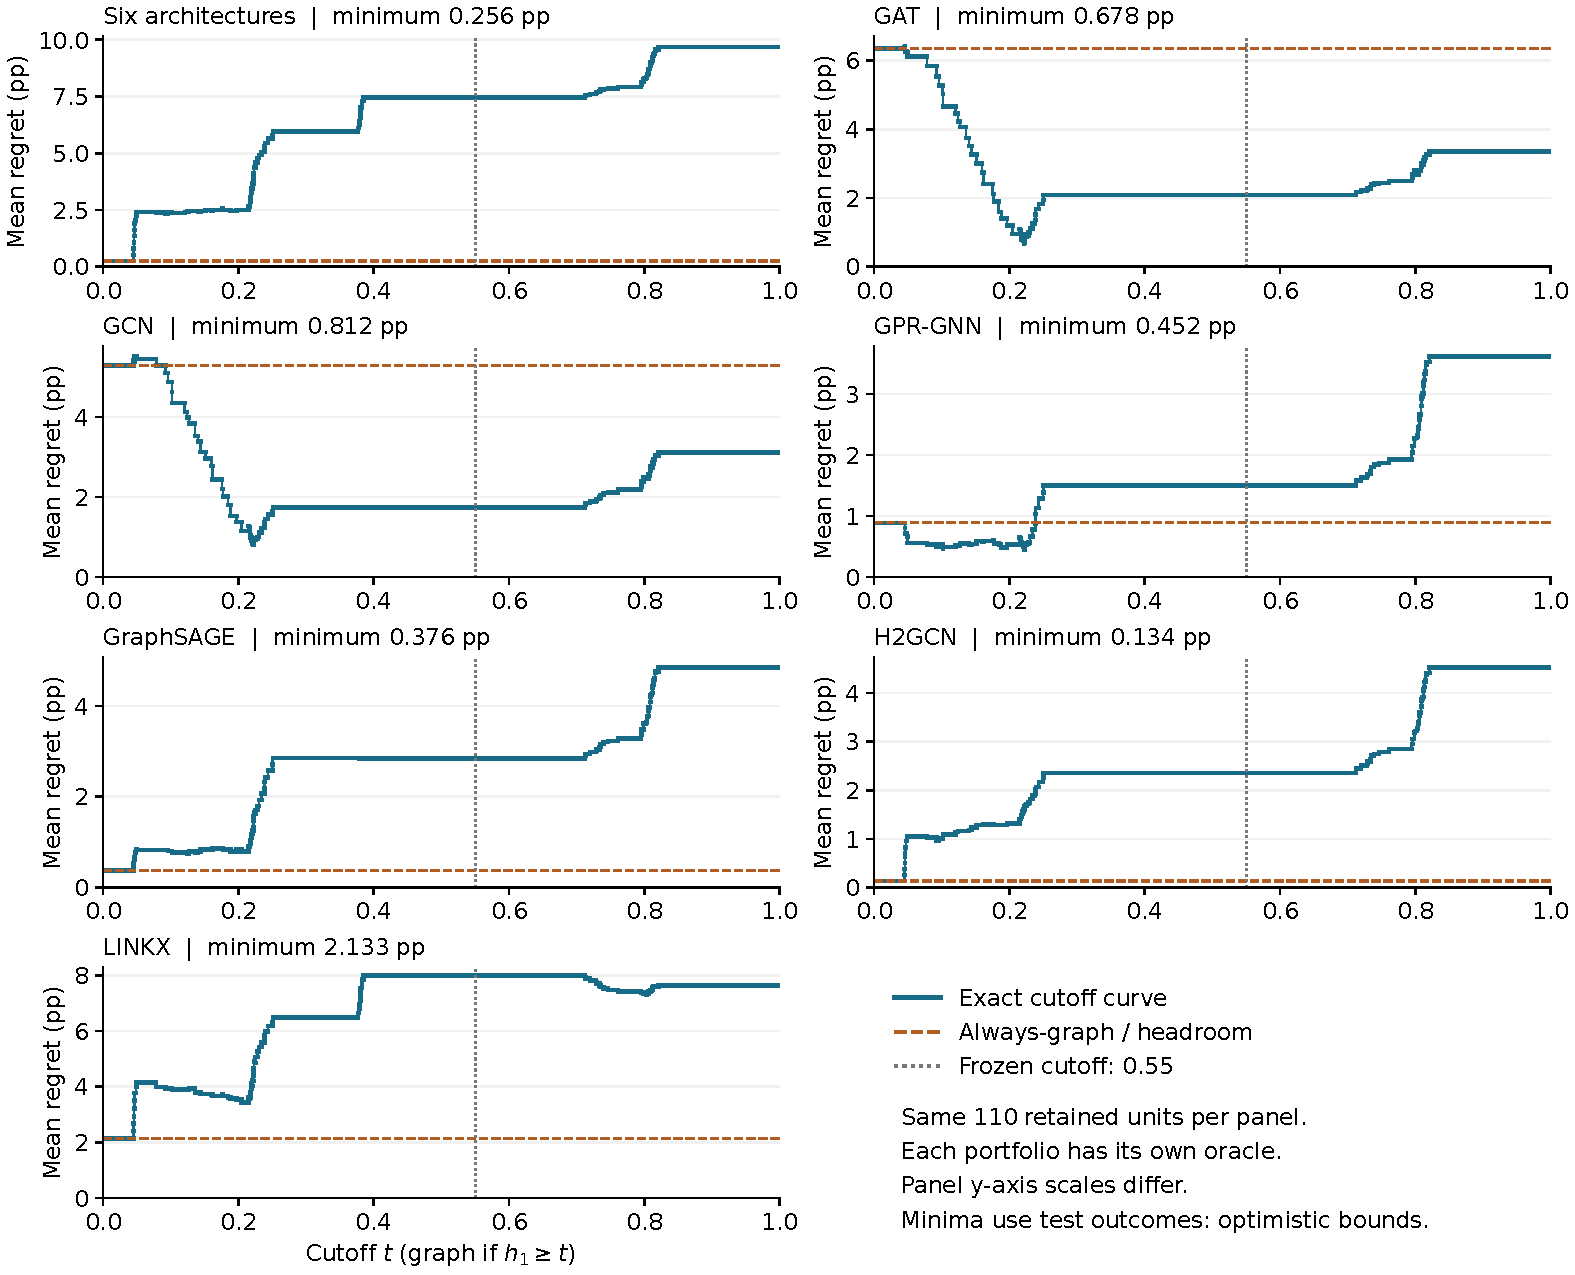
\includegraphics[width=\linewidth]{results/diagnostic/route_a_prospective_v2/analysis/threshold_headroom.pdf}
\caption{Exact one-sided homophily-cutoff curves from retained outcomes. The curves are constant on intervals ending at observed homophily values: equality selects graph. Vertical connectors guide the eye; full-precision endpoint inclusion is recorded in the supplement. Dashed horizontal lines show always-graph regret and dotted vertical lines show the frozen cutoff. Minima are selected using test outcomes, not held-out calibration. Panel vertical scales differ.}
\label{fig:threshold_headroom}
\end{figure}

\subsection{Action Counts and Raw Regret}
\label{app:action_confusion}

Table~\ref{tab:action_confusion} separates the practical-margin target from raw regret for the original full portfolio. The target is graph only when its test advantage exceeds one percentage point; raw regret instead measures any accuracy loss relative to the better recorded action. Thus a target-consistent MLP decision can still incur positive regret for a sub-margin graph advantage. The 19 and 30 graph-target counts are not the counts of positive-regret units, which are 23 and 32. All 40 explicit graph actions have zero regret in these records. This locates the observed policy losses without asserting that the rule cannot err when choosing graph in another setting.

\begin{table}[ht]
\centering
\caption{Full-portfolio action decomposition before the declared MLP fallback. Targets use the one-point margin; positive-regret counts use the raw accuracy difference. The contribution column divides each group's regret sum by all 110 units, so the entries add to the 7.457-point full-set regret.}
\label{tab:action_confusion}
\small
\setlength{\tabcolsep}{3.5pt}
\begin{tabular}{@{}lrrrrr@{}}
\toprule
Action & Units & Graph target & MLP target & Positive regret & Contribution (pp) \\
\midrule
Graph & 40 & 40 & 0 & 0 & 0.000 \\
MLP & 35 & 19 & 16 & 23 & 1.799 \\
Abstain $\to$ MLP & 35 & 30 & 5 & 32 & 5.658 \\
\midrule
Total & 110 & 89 & 21 & 55 & 7.457 \\
\bottomrule
\end{tabular}
\end{table}

\FloatBarrier
\section{Post-Hoc Training and Input-Parameterization Diagnostics}
\label{app:training_diagnostics}

We test whether reparameterizing the normalized features improves baseline performance on the two datasets in Appendix~\ref{sec:preprocessing_sensitivity}. These post-hoc experiments were designed after inspecting the earlier results and use training and validation labels only. They diagnose the baseline on the existing datasets without new test evaluations.

\subsection{Design and Information Scope}

Let $X$ be the raw feature matrix, $N$ the result of the unchanged PyG \texttt{NormalizeFeatures} transform, and $T$ the training-node index set. For a feature matrix $Z$, define
\[
  \mu_T(Z)=\frac{1}{|T|}\sum_{i\in T}Z_i,
  \qquad
  R_T(Z)=\sqrt{\frac{1}{|T|d}\sum_{i\in T}\|Z_i-\mu_T(Z)\|_2^2}.
\]
The added scale is the single scalar $a=R_T(X)/R_T(N)$, rather than a per-feature standardization. We compare $X$, $N$, $aN$, $N-\mu_T(N)$, and $a(N-\mu_T(N))$. The added mean and scale are fitted using training features without labels and then applied to all nodes. The underlying $N$ retains the frozen transductive transform, including its global feature-matrix minimum; the claim of training-only fitting applies to the added affine statistics. The approximate scales are 531 on Roman-empire and 376 on Amazon-ratings.

The first stage trains MLP under all five conditions and two weight decays, $5\times10^{-4}$ and zero. Two datasets, ten existing seeds, and four trials per condition give 200 selected records and 800 trials. The second stage retains raw, normalized, and centered-scaled inputs, fixes weight decay at $5\times10^{-4}$, and trains all seven original architectures: 420 selected records and 1,680 trials. Both stages retain hidden width 64, the original learning-rate/dropout grid, at most 500 epochs, patience 100, and the validation selection rule. Validation is used for both checkpoint/trial selection and these descriptive summaries; it is not an unbiased estimate of held-out test performance. The ten paired seeds measure within-dataset variation on the same two datasets.

\subsection{MLP Diagnosis}

\begin{table}[ht]
\centering
\caption{Post-hoc MLP input diagnosis at weight decay $5\times10^{-4}$. Entries are mean validation accuracy in percent, with sample standard deviation across ten seeds. These are selected validation results, not test results or population confidence intervals.}
\label{tab:mlp_parameterization}
\small
\begin{tabular}{@{}lrr@{}}
\toprule
Input & Roman-empire & Amazon-ratings \\
\midrule
Raw $X$ & $66.44\pm0.46$ & $41.84\pm0.50$ \\
Normalized $N$ & $16.75\pm4.20$ & $36.80\pm0.00$ \\
Scaled $aN$ & $41.25\pm1.61$ & $36.80\pm0.01$ \\
Centered $N-\mu_T(N)$ & $20.60\pm4.57$ & $36.80\pm0.00$ \\
Centered-scaled $a(N-\mu_T(N))$ & $66.45\pm0.44$ & $42.65\pm0.69$ \\
\bottomrule
\end{tabular}
\end{table}

Centering and scaling together recover approximately raw-feature MLP validation accuracy on Roman-empire and exceed it descriptively on Amazon-ratings (Table~\ref{tab:mlp_parameterization}). On Amazon-ratings, the normalized model predicts the training majority class for every validation node in all ten seeds, both with the original weight decay and with zero weight decay. Centering or scaling alone does not resolve this behavior under the original regularization, whereas their combination removes constant validation predictions in all ten seeds. On Roman-empire, five normalized-feature seeds predict only the majority class; predictions in the other five are nonconstant.

For nonzero $a$, the map from $N$ to $a(N-\mu_T(N))$ is invertible in exact arithmetic. An MLP with a biased first affine layer can represent the same functions under this change by reparameterizing that layer. The recovery shows that finite training and selection can respond to an information-preserving reparameterization. Optimization, regularization, activation dynamics, and early stopping are competing explanations that this design leaves unresolved. The invertibility argument relates the two normalized input maps; raw features and $N$ can differ in information content. Removing weight decay alone is insufficient. For centered-scaled Amazon-ratings, zero weight decay trades higher validation accuracy for higher validation cross-entropy.

\subsection{Extension to the Evaluated Architectures}

\begin{table}[ht]
\centering
\caption{The completed post-hoc architecture diagnosis: mean selected-checkpoint validation accuracy in percent over ten seeds, at weight decay $5\times10^{-4}$. N is \texttt{NormalizeFeatures}; CS is training-fitted centering and scalar scaling of N. Seed-level contrasts and standard deviations accompany the artifact. Values describe one completed training run and inherit the training-repeatability limitations discussed below.}
\label{tab:graph_parameterization}
\small
\begin{tabular}{@{}lrrrrrr@{}}
\toprule
& \multicolumn{3}{c}{Roman-empire} & \multicolumn{3}{c}{Amazon-ratings} \\
\cmidrule(lr){2-4}\cmidrule(l){5-7}
Model & Raw & N & CS & Raw & N & CS \\
\midrule
MLP & 66.44 & 16.75 & 66.45 & 41.84 & 36.80 & 42.65 \\
GCN & 50.93 & 20.45 & 50.71 & 43.76 & 36.80 & 44.52 \\
GAT & 46.15 & 15.11 & 42.53 & 44.36 & 36.80 & 44.21 \\
GraphSAGE & 78.36 & 21.34 & 78.51 & 47.09 & 36.80 & 48.93 \\
H2GCN & 81.21 & 28.34 & 81.07 & 46.69 & 36.91 & 47.56 \\
LINKX & 60.54 & 43.34 & 60.40 & 54.10 & 53.61 & 54.21 \\
GPR-GNN & 70.61 & 13.97 & 70.42 & 45.87 & 36.80 & 46.35 \\
\bottomrule
\end{tabular}
\end{table}

CS exceeds N in all 140 dataset--architecture--seed pairs (Table~\ref{tab:graph_parameterization}), a descriptive result on these dependent observations. The comparison with raw features varies by architecture: Roman-empire GAT is 3.62 percentage points worse on average under CS, with lower accuracy in all ten paired seeds. These validation results are analyzed separately from the earlier test accuracies. The first-layer reparameterization argument applies to MLP; functional equivalence for the graph architectures requires separate analysis.

\subsection{Record Integrity and Training Repeatability}
\label{app:training_reproducibility}

The completed records bind the raw-file hashes, split identifiers, transformed-feature hashes, training recipe, and executable source fingerprints. In the retained control comparisons, MLP selections reproduce across stages, with later replay metrics differing at most at floating-point scale. Graph retraining can differ in the tested settings: Roman-empire LINKX under N at seed 4 has validation accuracy 24.70\% in the earlier preprocessing run and 49.39\% in the completed architecture diagnosis, despite matching transformed inputs. The source snapshots and both original results are retained. The matching inputs locate the observed discrepancy in the training and selection process.

The initial architecture-diagnosis attempt stopped when a GAT checkpoint replay did not exactly match its recorded selection metric. A fresh run records the metric used for selection separately from the metric obtained when replaying the selected checkpoint. The new accounting preserves the selection rule and distinguishes checkpoint selection from replay. The failed attempt is archived separately from the completed 420-record run; the repeatability audit below examines training variability.

We then froze a bounded audit of 22 independent processes on Roman-empire. The core comparison repeats LINKX at normalized-input seed 4 for trials 001 and 003, each three times under default CUDA and three times under a deterministic CUDA configuration. Trial 001 uses learning rate 0.01 and dropout 0.7; trial 003 uses learning rate 0.005 and dropout 0.7. Each retains the original 500-epoch cap and patience 100. The deterministic configuration sets \texttt{CUBLAS\_WORKSPACE\_CONFIG=:4096:8} before importing PyTorch, enables deterministic algorithms, disables cuDNN benchmarking and TF32, and enables cuDNN determinism. We preserve initial and selected model states including buffers, random-state hashes, early logits and gradients, complete epoch histories, and repeated inference from each selected checkpoint.

\begin{table}[ht]
\centering
\caption{Independent-process LINKX audit on Roman-empire, normalized inputs, seed 4. Each row contains three repetitions of one fixed trial, not three different seeds or repeated four-trial model selection. Accuracy is the selected validation metric. Exact history and selected-state agreement is assessed within each row.}
\label{tab:training_reproducibility}
\small
\begin{tabular}{@{}llrl@{}}
\toprule
Trial & Backend configuration & Validation range (\%) & Histories/states identical \\
\midrule
001 & Default CUDA & 13.84--40.66 & No \\
003 & Default CUDA & 28.32--42.65 & No \\
001 & Deterministic CUDA & 13.84--13.84 & Yes \\
003 & Deterministic CUDA & 42.89--42.89 & Yes \\
\bottomrule
\end{tabular}
\end{table}

All 22 processes complete without test evaluation. In each default-CUDA core group, initial model states and random states agree, but logits, gradients, and updated weights already differ at epoch zero. Selected validation accuracy spans 26.82 and 14.33 percentage points for the two trials (Table~\ref{tab:training_reproducibility}). Under deterministic CUDA, each three-process group has identical full training histories and selected-state hashes. Two-process deterministic controls also agree exactly for LINKX raw and CS inputs, MLP normalized inputs, and GAT normalized inputs at seed 9; two 12-epoch CPU LINKX controls agree within the CPU setting. Repeated inference from the selected checkpoints and reconstruction of the saved model produce no class-prediction disagreements in this audit. Default CUDA still shows logit differences up to $1.53\times10^{-5}$ on fixed-checkpoint repeated inference, whereas the deterministic and CPU comparisons are exact.

The audit characterizes training repeatability under the tested configurations: it records large default-CUDA variability in the selected real-data condition and identical histories and selected states within the specified deterministic repeat groups. Repeatability does not ensure good optimization: deterministic trial 001 still has only 13.84\% validation accuracy. At seed 4 with that fixed trial, raw and CS LINKX accuracies are 60.09\% and 59.05\%, preserving the direction of the normalized-input deficit for that limited comparison. These are not replacements for the original four-trial selections or a rerun of all ten seeds. The backend intervention combines several settings, and trajectory hashing synchronizes CUDA and may affect scheduling. The original 770 benchmark records used an RTX 3070 Laptop GPU and PyTorch's CUDA 12.6 build; the added diagnoses and audit use an RTX 5060 and the CUDA 12.8 build. The original records do not include the detailed deterministic-backend flags recorded by this audit. These differences leave the responsible kernel and the causes of individual historical discrepancies unresolved. Repeatability across the original 11-dataset training runs and all 420 diagnosis records also remains unverified.

Baseline comparisons need both the preprocessing protocol and evidence of training repeatability. The findings here apply to the recorded configurations. Broader claims about preprocessing, model rankings, or effect sizes across backends and unseen datasets require independent evidence.

\FloatBarrier
% ============================================================
% Scoped aggregation discriminability analysis
% Target: ~4 pages
% ============================================================

\section{Scoped Mechanistic Context: Aggregation Discriminability}
\label{sec:snr}

We derive the effect of linear aggregation on class-conditional first and second moments in a binary fixed-degree surrogate. The exact calculation describes how feature strength, edge correlation, and degree jointly determine moment-based discriminability. It provides mechanistic context for the empirical audit under the stated conditional-neighbor model.

\begin{table}[t]
\centering
\caption{Key Notation Used in This Section}
\label{tab:notation}
\small
\begin{tabular}{@{}cl@{}}
\toprule
\textbf{Symbol} & \textbf{Definition} \\
\midrule
$\rho$ & Conditional neighbor-label correlation, $\rho\in[-1,1]$ \\
$d$ & Fixed number of aggregated neighbors \\
$s$ & Feature strength, $s=\mu^\top\Sigma^{-1}\mu$ \\
$\kappa$ & Exact discriminability ratio in Proposition~\ref{prop:fixed_degree} \\
$\alpha$ & Weight on the center-node feature, $\alpha\in[0,1]$ \\
$\mathcal{D}(Z)$ & Moment-based Mahalanobis discriminability of $Z$ \\
$\Delta_Z$ & Class separation, $\mathbb{E}[Z|Y=+1] - \mathbb{E}[Z|Y=-1]$ \\
$\Sigma_Z$ & Within-class covariance, $\mathrm{Cov}(Z|Y)$ \\
\bottomrule
\end{tabular}
\end{table}

\subsection{Problem Setup}

Let the center label be $Y_v\in\{-1,+1\}$ with equal class prior and let
\begin{equation}
    X_v=Y_v\mu+\varepsilon_v,
    \qquad \varepsilon_v\sim\mathcal{N}(0,\Sigma),
\end{equation}
where $\Sigma\succ0$, $\mu\neq0$, and noises are independent across nodes. Conditional on $Y_v=y$, the $d\geq1$ neighbor labels are independent and satisfy
\begin{equation}
    \mathbb{P}(Y_i=y\mid Y_v=y)=\frac{1+\rho}{2}.
\end{equation}
Thus $\mathbb{E}[Y_i\mid Y_v=y]=\rho y$ and $\operatorname{Var}(Y_i\mid Y_v=y)=1-\rho^2$. In a balanced binary graph with a uniform conditional neighbor mechanism, $\rho$ corresponds to $2h-1$; the derivation itself is conditional and does not replace a random graph degree by its mean.

\begin{definition}[Moment-Based Discriminability]
\label{def:discriminability}
Let the two classes share a nonsingular conditional covariance $\Sigma_Z$. We define the moment-based discriminability of representation $Z$ as
\begin{equation}
    \mathcal{D}(Z) := \Delta_Z^\top \Sigma_Z^{-1} \Delta_Z
\end{equation}
where $\Delta_Z = \mathbb{E}[Z|Y=+1] - \mathbb{E}[Z|Y=-1]$. This quantity uses only the first two conditional moments. It is not, in general, a distance between the full class-conditional distributions.
\end{definition}

\subsection{Exact Fixed-Degree Calculation}

Conditional on a center label $Y_v=y$, let $Y_1,\ldots,Y_d$ be independent neighbor labels satisfying $\mathbb{P}(Y_i=y\mid Y_v=y)=(1+\rho)/2$. Let $X_i=Y_i\mu+\varepsilon_i$, where the $\varepsilon_i\sim\mathcal{N}(0,\Sigma)$ are independent of all labels, and define $A_v=d^{-1}\sum_{i=1}^d X_i$.

\begin{proposition}[Exact Fixed-Degree Discriminability]
\label{prop:fixed_degree}
For $s=\mu^\top\Sigma^{-1}\mu>0$, the conditional moments and discriminability ratio are
\begin{align}
    \mathbb{E}[A_v\mid Y_v=y] &= \rho y\mu,\\
    \operatorname{Cov}(A_v\mid Y_v=y)
        &= \frac{1}{d}\left(\Sigma+(1-\rho^2)\mu\mu^\top\right),\\
    \kappa(d,\rho,s)
        :=\frac{\mathcal{D}(A)}{\mathcal{D}(X)}
        &=\frac{\rho^2d}{1+(1-\rho^2)s}.
\end{align}
\end{proposition}

\begin{proof}


Since $\mathbb{E}[Y_i\mid Y_v=y]=\rho y$ and
$\operatorname{Var}(Y_i\mid Y_v=y)=1-\rho^2$, independence gives the first two identities. Moreover, $\Delta_X=2\mu$, $\mathcal{D}(X)=4s$, and $\Delta_A=2\rho\mu$. Applying the Sherman--Morrison identity,
\begin{equation}
 \mu^\top\left(\Sigma+(1-\rho^2)\mu\mu^\top\right)^{-1}\mu
 =\frac{s}{1+(1-\rho^2)s}.
\end{equation}
Substitution yields the stated ratio.
\end{proof}

\subsection{Center-Feature and Neighbor Mixing}

To examine retention of the center feature, we use the linear surrogate
\begin{equation}
    Z_{\alpha,v}=\alpha X_v+(1-\alpha)A_v,
    \qquad \alpha\in[0,1].
    \label{eq:self_neighbor_operator}
\end{equation}
The scalar $\alpha$ is a prescribed mixing weight; it is not identified with a learned GCN coefficient.

\begin{proposition}[Exact Self--Neighbor Mixing Discriminability]
\label{prop:self_neighbor_mixing}
Under the fixed-degree model above, assume that the center-feature noise is conditionally independent of all neighbor labels and features. Define
\begin{align}
    m_\alpha &= \alpha+(1-\alpha)\rho,\\
    c_\alpha &= \alpha^2+\frac{(1-\alpha)^2}{d},\\
    q_\alpha &= \frac{(1-\alpha)^2(1-\rho^2)}{d}.
\end{align}
Then
\begin{align}
    \mathbb{E}[Z_{\alpha,v}\mid Y_v=y]
        &=m_\alpha y\mu,\\
    \operatorname{Cov}(Z_{\alpha,v}\mid Y_v=y)
        &=c_\alpha\Sigma+q_\alpha\mu\mu^\top,
\end{align}
and the exact moment-based discriminability ratio is
\begin{align}
    \kappa_\alpha(d,\rho,s)
    &:=\frac{\mathcal{D}(Z_\alpha)}{\mathcal{D}(X)} \notag\\
    &=\frac{[\alpha+(1-\alpha)\rho]^2}
    {\alpha^2+(1-\alpha)^2/d
    +[(1-\alpha)^2/d](1-\rho^2)s}.
    \label{eq:kappa_alpha}
\end{align}
\end{proposition}

\begin{proof}
Conditional independence makes the center and neighbor covariance contributions additive, which gives the stated mean and covariance. For
$B=c_\alpha\Sigma+q_\alpha\mu\mu^\top$, the Sherman--Morrison identity gives
\begin{equation}
    \mu^\top B^{-1}\mu=\frac{s}{c_\alpha+q_\alpha s}.
\end{equation}
Since the class-mean difference is $2m_\alpha\mu$, we have
$\mathcal{D}(Z_\alpha)=4m_\alpha^2s/(c_\alpha+q_\alpha s)$. Dividing by $\mathcal{D}(X)=4s$ proves~\eqref{eq:kappa_alpha}.
\end{proof}

The boundary cases provide checks on the formula. Setting $\alpha=0$ recovers Proposition~\ref{prop:fixed_degree}; setting $\alpha=1$ gives $\kappa_\alpha=1$; and $|\rho|=1$ removes label-mixture covariance. A negative $\rho$ can also cancel the center and neighbor class means when $m_\alpha=0$, showing why self-loops do not uniformly prevent damage.

\begin{corollary}[Discriminability Transition]
\label{cor:threshold}
In the fixed-degree model, aggregation improves Mahalanobis discriminability exactly when
\begin{align}
    \kappa>1
    &\iff \rho^2 > \frac{1+s}{d+s}.
\end{align}
Thus the transition depends on feature strength as well as degree and edge correlation. The simpler condition $\rho^2d>1$ is recovered only as $s\to0$.
\end{corollary}

\begin{table}[t]
\centering
\caption{Exact Discriminability-Loss Region Depends on Feature Strength}
\label{tab:threshold}
\begin{tabular}{@{}ccc@{}}
\toprule
$(d,s)$ & Boundary $|2h-1|$ & Loss Region ($h$) \\
\midrule
$(10,0^+)$ & 0.316 & (0.34, 0.66) \\
$(10,1)$ & 0.426 & (0.29, 0.71) \\
$(10,4)$ & 0.598 & (0.20, 0.80) \\
$(20,1)$ & 0.309 & (0.35, 0.65) \\
\bottomrule
\end{tabular}
\end{table}

In Table~\ref{tab:threshold}, the first row is the limit as $s\to0^+$; the ratio is undefined when both class representations have zero discriminability. Stronger self-feature separation increases the label-mixture penalty and widens the region where neighbor-only aggregation loses moment-based discriminability.

\subsection{Approximation Regime}

The exact ratio satisfies
\begin{equation}
 \kappa=\frac{\rho^2d}{1+\eta}\leq\rho^2d,
 \qquad \eta=(1-\rho^2)s.
\end{equation}
For $\rho\neq 0$, the exact ratio falls below the approximation by the fraction
$(\rho^2d-\kappa)/(\rho^2d)=\eta/(1+\eta)$, while the approximation overstates the exact value by $(\rho^2d-\kappa)/\kappa=\eta$. This makes the required feature-noise-dominance regime explicit and does not invoke an asymptotic $o(1)$ term.

\subsection{Direct Moment Validation}

We test the implemented formulas on a frozen simulation grid. The grid uses dimension four, identity covariance, $d\in\{2,5,10,20\}$, $\rho\in\{-0.8,-0.4,0,0.4,0.8\}$, $s\in\{0.1,0.5,1,4\}$, and $\alpha\in\{0,0.25,0.5,0.75,1\}$. It contains 400 configurations, five seeds (202608080--202608084), and 5,000 samples per class. Percentile-bootstrap intervals use 5,000 resamples of configuration--seed records (base seed 20260808); per-strength intervals increment that seed in ascending strength order. These intervals describe the fixed grid, not real-graph generalization. All 2,000 configuration--seed records completed successfully, retaining empirical moments, exact predictions, environment, and source commit. Across 1,920 records with a nonzero exact ratio, the median absolute relative error between the empirical estimate and $\kappa_\alpha$ is 0.94\%. Its descriptive 95\% percentile-bootstrap interval is 0.86--1.05\%. In the neighbor-only slice, the simplified $\rho^2d$ approximation has median absolute error 0.293 (0.242--0.365); its overstatement increases with feature strength.

\begin{figure}[t]
\centering
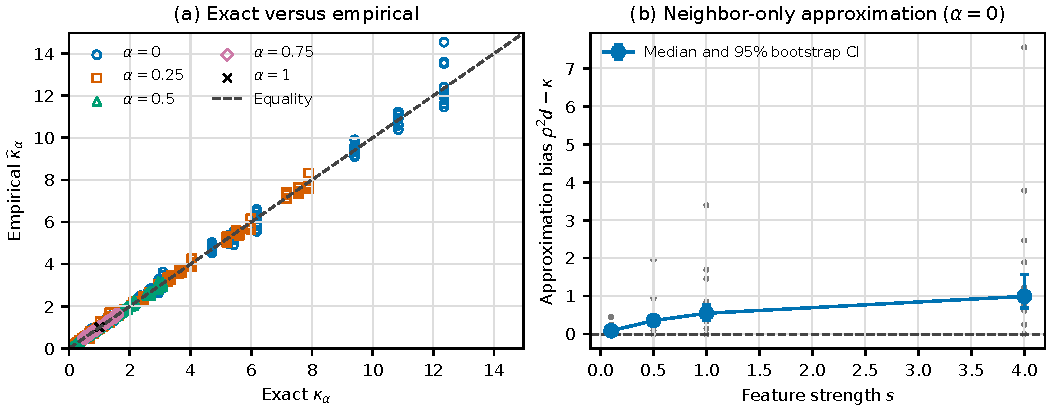
\includegraphics[width=\linewidth]{results/discriminability/route_a_grid_v1/summary/validation_figure}
\caption{Frozen moment validation. Left: empirical and exact $\kappa_\alpha$. Right: signed error of the neighbor-only $\rho^2d$ approximation. Grey points are individual configuration--seed records (100 at each feature strength, with overlapping values), not configuration means. Blue markers and bars show the median and its descriptive 95\% percentile-bootstrap interval, resampling those records within each strength.}
\label{fig:direct_discriminability_validation}
\end{figure}

The simulation checks the implemented first- and second-moment formulas across the prescribed grid.

\subsection{Relation to tree broadcasting}

The product ``branching factor $\times$ squared label correlation'' also appears in classical tree broadcasting and reconstruction. For a regular tree with forward branching factor $b$, the Kesten--Stigum quantity is $b\rho^2$~\citep{kesten1966additional,mossel2015reconstruction}. Here $b=q-1$ for a $q$-regular undirected tree, whereas a Poisson Galton--Watson limit with mean offspring $k$ uses $b=k$. The weak-feature limit of our one-hop ratio has this established form. In particular, $d$ in Proposition~\ref{prop:fixed_degree} is a fixed one-hop neighbor count and must not be interchanged with either forward degree without an explicit coupling. Ordinary finite-depth GNNs also reuse neighborhoods and may include self-loops, normalization, nonlinearities, attention, and learned transformations. We therefore derive no Kesten--Stigum condition for GNN depth or architecture. Recent finite-depth CSBM analysis likewise finds Gaussian-mixture embeddings and depth behavior more complex than a single-Gaussian account~\citep{pmlr-v269-dalle25a}.

\subsection{Multiclass and multilayer models}

A multiclass extension requires a class-transition matrix and the arrangement of class feature means. Scalar homophily can conceal both the mixed class pairs and their feature geometry. Extending the calculation to a practical GCN would also require variable degree, self-loop normalization, learned transformations, nonlinearities, and neighborhood reuse across layers. Proposition~\ref{prop:self_neighbor_mixing} addresses the prescribed self-feature weight within the linear surrogate.

\subsection{Scope and Random-Degree Extension}

The class-conditional distribution of $A_v$ is generally a Gaussian mixture because the neighbor labels are random. Therefore the Gaussian Bayes-error formula for a single Gaussian class-conditional model must not be applied to $A_v$ solely from its first two moments. Proposition~\ref{prop:fixed_degree} concerns Mahalanobis discriminability only.

For sparse CSBM, degree is random. Conditional on $D_v=m>0$, Proposition~\ref{prop:fixed_degree} applies with $d=m$. An unconditional calculation would need to specify the treatment of isolated nodes and average over the degree-conditioned mixture. Replacing $D_v$ by its mean is not exact; the fixed-degree result supplies no finite-$n$ error rates for that extension.

\FloatBarrier
\section{Execution Provenance and Supporting Displays}
\label{app:execution_details}

\subsection{Protocol Amendments and Provenance}

The execution history contains two documented amendments. First, the v1 feasibility run stops before model training on Texas because one class contains a single node and cannot populate the frozen three-way split. Before comparative assembly or evaluation, an outcome-independent eligibility amendment excludes Texas, assigns a new run identifier, and restarts all remaining datasets from zero without changing models, splits, seeds, thresholds, metrics, or inference. Second, after a blinded wall-clock timeout on Squirrel, an execution-only amendment increases the per-dataset limit from 30 to 90 minutes. No comparative outcome is inspected, and all scientific settings remain unchanged. The completed v2 artifacts retain the amendments and exclude the aborted v1 records from analysis.

Here ``prospective'' refers specifically to newly generated records for the pre-specified primary analysis, produced after the specification and scoring implementation were frozen. Legacy aggregate results inspected during exploratory work are not part of this analysis because they lack consistent paired outcomes and decision-time provenance. The public release provides the frozen snapshot, file digests, and mappings to execution provenance, but it does not expose the private predecessor history; the auditable claim is therefore about the released primary run rather than the entire earlier research timeline.

\subsection{Threshold Provenance}

The exact Combined thresholds were not inherited verbatim from an earlier committed rule or derived through a prospective threshold sweep. They first appeared in the frozen specification and scorer after legacy aggregate inspection and before the primary records. Dated source provenance remains in the author archive. The public snapshot documents the released run, while the private predecessor history remains inaccessible.

\subsection{Regret--Coverage Display}
\label{app:coverage_display}

\begin{figure}[t]
\centering
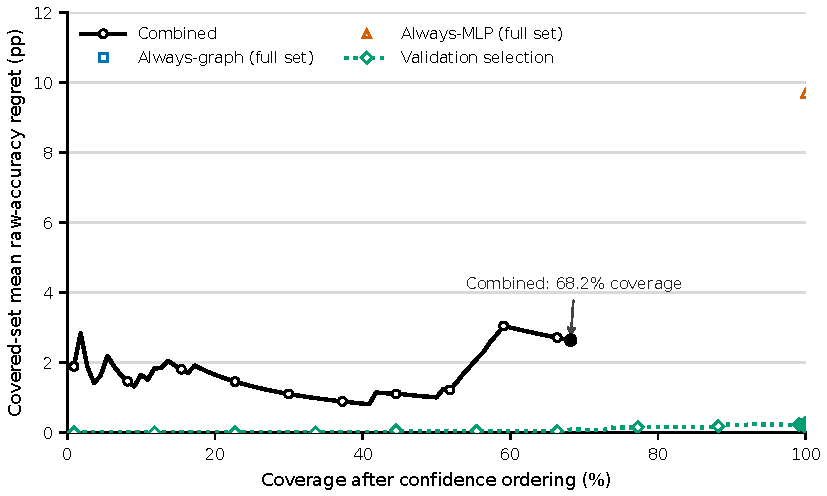
\includegraphics[width=0.82\linewidth]{results/diagnostic/route_a_prospective_v2/analysis/prospective_regret_coverage.pdf}
\caption{Descriptive regret--coverage display from the frozen confidence scores. For Combined and validation selection, coverage increases as lower-confidence eligible decisions enter. Always-graph and always-MLP have constant confidence and therefore appear only as full-set endpoints. The ordinate is covered-set mean raw-accuracy regret, not selection error under the one-point target margin. The Combined curve ends at 68.2\% because 35 units abstain and fallback decisions are not added to this display. The pre-specified primary analysis remains full-set regret with dataset-level inference.}
\label{fig:regret_coverage}
\end{figure}

Figure~\ref{fig:regret_coverage} shows the precomputed descriptive curves for Combined and validation selection, together with the two constant policies at their identifiable full-set endpoints. Raising confidence within the Combined rule does not reveal a sustained regret region comparable to the low-regret reference policies: its final covered-set regret is 2.64 points at 68.2\% coverage, compared with full-set regrets of 0.26 for always-graph and 0.22 for validation selection. This display is a sensitivity summary only and does not replace the predeclared full-set comparison.

\FloatBarrier
\clearpage
\section{Post-Hoc Input-Parameterization Retraining and MLP-Budget Extension}
\label{app:mlp_budget}

This appendix supplements Sections~\ref{sec:input_robustness} and~\ref{sec:mlp_budget}. It concerns three separate record sets: the frozen benchmark, which is unchanged; a post-hoc retraining of all seven architectures on the same 11 datasets and 110 splits under two inputs (1,540 records, 4 trials per architecture); and a post-hoc extension of the MLP search within that retraining. Numbers from different record sets are not pooled, and no number below revises a frozen-benchmark result.

\subsection{Protocol and Record Integrity}

The extension covers 220 MLP units. Each inherits the 4 trials of the matching retraining record, including their saved checkpoints, and adds 20 trials (4,400 in total); every trial uses the unit's original seed initialization. Selection uses validation accuracy, then validation loss, then trial identifier, over all 24 candidates. In 75 units an inherited trial remains selected and in 145 a new trial is selected. The selected checkpoint is reloaded and evaluated on the test split exactly once, also when an inherited trial remains selected; earlier test results are kept only as historical evidence and are never assigned to a different winner. Test-once violations: 0. The graph records and all decision rules are those of the retraining, and the extension design, including two additional published statistics, was fixed after inspecting partial results of that retraining.

The first execution attempt of one unit failed before any training because its worker started in an environment without GPU support. That attempt and its budget charge are retained as failed; after a recorded review, a single retry in the specified environment produced the unit's only record. Decision scores are computed with the analysis code in the accompanying archive; the frozen analysis outputs, including all intervals in Table~\ref{tab:mlp_budget_intervals}, were reproduced exactly from the validated records.

\subsection{Published Statistics and Study-Specific Calibration}

We implement adjusted homophily and the uniform-edge label informativeness of \citet{platonov2023characterizing} on the subgraph induced by training nodes. For this statistic only, edges are made undirected, deduplicated, and stripped of self-loops; model-training graphs remain unchanged. Let $P_{ij}$ be the fraction of ordered edge-endpoint label pairs of classes $i,j$, and $q_i=\sum_jP_{ij}$ the endpoint class distribution. The implemented statistics are
\begin{align}
h_{\mathrm{adj}}&=\frac{\sum_iP_{ii}-\sum_iq_i^2}{1-\sum_iq_i^2},\\
\mathrm{LI}_{\mathrm{edge}}&=\frac{\sum_{i,j:P_{ij}>0}P_{ij}\log(P_{ij}/(q_iq_j))}
{-\sum_{i:q_i>0}q_i\log q_i}.
\end{align}
A statistic is unavailable if there are no training edges or only one endpoint class; its policy then abstains with the declared MLP fallback. Neither validation nor test labels enter these statistics.

For each of these two published statistics, input, MLP budget, and graph portfolio, leave-one-dataset-out calibration chooses a graph-if-score-at-least-threshold rule using only the other ten datasets. Candidate thresholds comprise midpoints between their distinct observed scores plus constant-graph and constant-MLP policies. Calibration minimizes equal-weight dataset mean regret on selected-model test outcomes from those ten datasets, used as meta-training targets; ties within $10^{-12}$ choose the smallest threshold. The held-out dataset's scores and outcomes do not determine the candidates or their selection. Constant policies retain the missing-statistic abstention rule. All folds, scores, and decisions are retained. Ordinary $h_1$ retains the fixed grid in Section~\ref{sec:calibrated_threshold}, including its constant policies. The comparisons therefore concern complete statistic-plus-calibration policies and do not isolate the effect of the statistic alone. This post-hoc adaptation evaluates the published statistics as decision inputs and does not reproduce an original published selector.

\subsection{Policy Regrets}

\begin{table}[tbp]
\centering
\caption{Full-set mean regret (percentage points) of all evaluated policies for the six-architecture portfolio in the post-hoc retraining, with four and 24 MLP trials. The three calibrated rules fit thresholds on the other ten datasets; ordinary $h_1$ uses the fixed 0.01 grid, and the two additional statistics use fold-specific score midpoints; the two published statistics are not reproductions of their authors' selectors. Descriptive values; no interval was specified for the 24-trial extension.}
\label{tab:mlp_budget_policies}
\small
\begin{tabular}{@{}lrrrr@{}}
\toprule
 & \multicolumn{2}{c}{$N$} & \multicolumn{2}{c}{CS} \\
\cmidrule(lr){2-3}\cmidrule(lr){4-5}
Policy & 4 trials & 24 trials & 4 trials & 24 trials \\
\midrule
Combined & 7.60 & 6.72 & 6.22 & 5.75 \\
Always-graph & 0.40 & 0.44 & 0.45 & 0.53 \\
Validation selection & 0.32 & 0.21 & 0.20 & 0.28 \\
Always-MLP & 9.81 & 8.47 & 7.99 & 7.48 \\
Homophily only & 7.60 & 6.72 & 6.22 & 5.75 \\
Degree only & 6.36 & 5.14 & 4.24 & 3.88 \\
Homophily + degree & 5.94 & 5.14 & 4.11 & 3.81 \\
Two-hop only & 8.59 & 7.33 & 6.88 & 6.51 \\
Random 50/50 & 5.11 & 4.46 & 4.22 & 4.01 \\
\midrule
Calibrated $h_1$ (LODO) & 2.84 & 2.04 & 1.80 & 1.88 \\
Adjusted homophily (LODO) & 0.27 & 0.34 & 0.10 & 0.15 \\
Edge label informativeness (LODO) & 2.36 & 0.44 & 2.53 & 2.59 \\
\bottomrule
\end{tabular}
\end{table}

\begin{table}[tbp]
\centering
\caption{Combined/always-graph mean regret (percentage points) for single-architecture graph actions in the post-hoc retraining. Each row has its own oracle; these records are separate from Table~\ref{tab:equal_budget}.}
\label{tab:mlp_budget_single}
\small
\begin{tabular}{@{}lrrrr@{}}
\toprule
 & \multicolumn{2}{c}{$N$} & \multicolumn{2}{c}{CS} \\
\cmidrule(lr){2-3}\cmidrule(lr){4-5}
Graph action & 4 trials & 24 trials & 4 trials & 24 trials \\
\midrule
GCN & 1.78/5.07 & 1.70/5.91 & 3.83/7.24 & 3.50/7.47 \\
GAT & 2.09/6.25 & 2.34/7.41 & 3.96/9.00 & 3.68/9.27 \\
GPR-GNN & 1.47/1.00 & 1.36/1.81 & 3.17/0.74 & 2.78/0.90 \\
GraphSAGE & 2.95/0.44 & 2.39/0.79 & 4.36/1.13 & 3.83/1.15 \\
H2GCN & 2.51/0.17 & 1.68/0.25 & 3.50/0.36 & 3.01/0.42 \\
LINKX & 8.09/2.74 & 7.30/2.87 & 4.44/3.44 & 3.95/3.50 \\
\bottomrule
\end{tabular}
\end{table}

Across all 63 subsets, the portfolios favoring Combined are GAT, GCN, GCN+GAT with $N$ and four MLP trials; GAT, GCN, GCN+GAT, GPR-GNN with $N$ and 24 trials; and GAT, GCN, GCN+GAT with CS at both budgets. After excluding Cornell and Wisconsin, only GPR-GNN with $N$ and 24 trials still favors Combined.

\subsection{Intervals Specified for the Retraining}

The retraining's frozen analysis configuration specifies dataset-bootstrap intervals for the eight comparisons with Combined and for the CS-minus-$N$ contrasts: 10,000 resamples of the 11 equal-weight dataset means, 95\% percentile intervals, without multiplicity adjustment. They apply only to the four-trial records; none was specified or computed for the 24-trial extension.

\begin{table}[tbp]
\centering
\caption{Specified dataset-bootstrap intervals for the four-trial retraining, six-architecture portfolio. Upper panel: policy minus Combined mean regret (percentage points). Lower panel: CS minus $N$ equal-weight dataset means (percentage points). Unadjusted, post hoc, and descriptive.}
\label{tab:mlp_budget_intervals}
\small
\begin{tabular}{@{}lrrrr@{}}
\toprule
 & \multicolumn{2}{c}{$N$} & \multicolumn{2}{c}{CS} \\
\cmidrule(lr){2-3}\cmidrule(lr){4-5}
Difference & Mean & 95\% interval & Mean & 95\% interval \\
\midrule
Always-graph $-$ Combined & $-$7.20 & [$-$13.67, $-$1.39] & $-$5.78 & [$-$11.23, $-$0.90] \\
Validation $-$ Combined & $-$7.29 & [$-$13.64, $-$1.53] & $-$6.03 & [$-$11.47, $-$1.23] \\
Always-MLP $-$ Combined & 2.21 & [0.38, 4.71] & 1.77 & [0.19, 4.11] \\
\midrule
CS $-$ $N$ & \multicolumn{2}{r}{Mean} & \multicolumn{2}{r}{95\% interval} \\
\midrule
Selected-MLP accuracy & \multicolumn{2}{r}{+5.94} & \multicolumn{2}{r}{[0.70, 15.01]} \\
Selected-graph accuracy & \multicolumn{2}{r}{+4.08} & \multicolumn{2}{r}{[0.22, 10.99]} \\
Combined regret & \multicolumn{2}{r}{$-$1.38} & \multicolumn{2}{r}{[$-$3.95, 0.40]} \\
Combined $-$ always-graph regret & \multicolumn{2}{r}{$-$1.43} & \multicolumn{2}{r}{[$-$3.92, 0.43]} \\
\bottomrule
\end{tabular}
\end{table}

\subsection{Selected MLP Accuracy and Input Contrast by Dataset}

\begin{table}[tbp]
\centering
\caption{Mean selected-MLP test accuracy (\%) over ten seeds in the post-hoc retraining, and the CS-minus-$N$ paired difference with 24 trials (mean, median, and seeds with CS higher/lower/tied). Descriptive values.}
\label{tab:mlp_budget_datasets}
\scriptsize
\setlength{\tabcolsep}{3.2pt}
\begin{tabular}{@{}lrrrrrrr@{}}
\toprule
 & \multicolumn{2}{c}{$N$} & \multicolumn{2}{c}{CS} & \multicolumn{3}{c}{CS $-$ $N$, 24 trials} \\
\cmidrule(lr){2-3}\cmidrule(lr){4-5}\cmidrule(lr){6-8}
Dataset & 4 & 24 & 4 & 24 & Mean & Median & H/L/T \\
\midrule
Cora & 76.37 & 76.35 & 75.86 & 75.66 & $-$0.69 & $-$0.46 & 1/9/0 \\
CiteSeer & 72.43 & 72.86 & 73.40 & 73.44 & +0.58 & +0.52 & 8/1/1 \\
PubMed & 87.53 & 87.41 & 88.09 & 88.08 & +0.67 & +0.71 & 10/0/0 \\
Wisconsin & 85.28 & 85.09 & 88.11 & 88.49 & +3.40 & +2.83 & 6/1/3 \\
Cornell & 76.00 & 76.00 & 78.75 & 78.75 & +2.75 & +3.75 & 7/2/1 \\
Chameleon & 46.51 & 47.93 & 47.52 & 48.85 & +0.92 & $-$0.11 & 4/5/1 \\
Squirrel & 31.22 & 31.07 & 30.90 & 31.20 & +0.13 & +0.05 & 5/3/2 \\
Actor & 37.97 & 37.77 & 37.21 & 37.27 & $-$0.50 & $-$0.53 & 2/7/1 \\
Roman-empire & 16.71 & 25.91 & 66.09 & 66.06 & +40.15 & +40.13 & 10/0/0 \\
Amazon-ratings & 36.76 & 36.76 & 41.98 & 45.99 & +9.22 & +9.31 & 10/0/0 \\
Coauthor-CS & 89.76 & 94.46 & 93.99 & 94.60 & +0.14 & +0.07 & 7/2/1 \\
\bottomrule
\end{tabular}
\end{table}

Leaving out one dataset at a time, the mean CS-minus-$N$ difference with 24 trials ranges from 1.66 to 5.75 points, and CS remains higher on 8 or 9 of the remaining ten datasets. The minimum occurs when Roman-empire is omitted; the remaining 100 paired seeds then split 60/30/10 (CS higher/lower/tied), with median 0.31 points. On Chameleon the mean and median differences have opposite signs. The input effect is therefore dataset-dependent, and no claim of consistent improvement is made.

\subsection{Amazon-ratings and Roman-empire with Normalized Features}

On Amazon-ratings with $N$, the selected test accuracy is identical in all ten seeds at both budgets: 1,802 correct of 4,902 test nodes in every seed; each test split contains exactly 1,802 majority-class nodes, so the observed accuracy equals the majority-class proportion of the test split. The ten selected checkpoints are distinct (10 different files), all 24 trials of every seed reach the same selected validation accuracy, no epoch of any trial exceeds the majority-class validation proportion, and the mean selected validation cross-entropy (1.4108) is close to the entropy of the class prior (1.4111). This behavior is consistent with majority-class collapse, which Appendix~\ref{app:training_diagnostics} observed directly as majority-class validation predictions in a separate run. The extension records store accuracies and checkpoints but not prediction vectors, so they do not verify constant predictions directly, and the cause of the collapse is not identified.

On Roman-empire with $N$, mean selected-MLP test accuracy is 16.71\% with four trials and 25.91\% with 24 (range 25.57--26.12\%). The number of seeds whose selected validation accuracy lies at the majority-class rate falls from 5 to 0. With CS the mean is 66.06\%, higher in 10 of 10 seeds by 39.64 to 40.57 points, so no single seed drives the dataset difference. The data binding, splits, transformed inputs, metric, and execution environment of every record match the frozen contract; we treat the low accuracy as a valid result of this input and training configuration, not as a pipeline failure.

\subsection{Dataset Exclusion and Abstention Fallback}
\label{sec:retraining_fallback}

A separate post-hoc reanalysis of the four-trial retraining crosses three abstention fallbacks with all datasets, joint Chameleon/Squirrel exclusion, joint Cornell/Wisconsin exclusion, and each single-dataset omission. It evaluates the full portfolio, GCN, GAT, and their pair, yielding 336 condition--portfolio--exclusion--fallback cases. Only Combined's abstentions change with fallback; explicit actions and other policies retain their recorded decisions. The analysis reconstructs the earlier unrestricted scores and intervals before scoring these cases.

\begin{table}[tbp]
\centering
\caption{Post-hoc fallback and dataset-exclusion sensitivity in the four-trial retraining, six-architecture portfolio. Regrets are percentage points; $\Delta$ is Combined minus always-graph. These are separate records from Table~\ref{tab:fallback_sensitivity} and are not the 24-trial extension. Ch./Sq. denotes Chameleon and Squirrel.}
\label{tab:retraining_fallback}
\small
\setlength{\tabcolsep}{3.2pt}
\begin{tabular}{@{}lllrrr@{}}
\toprule
Input & Datasets & Fallback & Combined & Always-graph & $\Delta$ \\
\midrule
N & All 11 & MLP & 7.605 & 0.404 & +7.200 \\
N & All 11 & Graph & 1.747 & 0.404 & +1.343 \\
N & All 11 & Validation & 1.730 & 0.404 & +1.326 \\
N & Exclude Ch./Sq. & MLP & 5.079 & 0.494 & +4.584 \\
N & Exclude Ch./Sq. & Graph & 0.308 & 0.494 & -0.187 \\
N & Exclude Ch./Sq. & Validation & 0.287 & 0.494 & -0.207 \\
\midrule
CS & All 11 & MLP & 6.223 & 0.448 & +5.775 \\
CS & All 11 & Graph & 4.122 & 0.448 & +3.674 \\
CS & All 11 & Validation & 4.136 & 0.448 & +3.688 \\
CS & Exclude Ch./Sq. & MLP & 3.022 & 0.547 & +2.475 \\
CS & Exclude Ch./Sq. & Graph & 3.005 & 0.547 & +2.457 \\
CS & Exclude Ch./Sq. & Validation & 3.022 & 0.547 & +2.475 \\
\bottomrule
\end{tabular}
\end{table}

Under the declared MLP fallback, every single-dataset omission retains Combined's higher full-portfolio regret: the excess ranges from 5.240 to 8.046 points under $N$ and from 4.057 to 6.636 under CS. Joint Cornell/Wisconsin exclusion reverses the favorable default-fallback averages for GCN, GAT, and their pair under both inputs.

The combined fallback/exclusion change has a different outcome. Under $N$, graph fallback and Chameleon/Squirrel exclusion give Combined 0.308 points against always-graph's 0.494; validation fallback gives 0.287 (Table~\ref{tab:retraining_fallback}). For graph fallback, the always-graph-minus-Combined dataset-bootstrap interval is [0.000, 0.464] points, with raw sign-flip $p=0.25$ and within-case Holm $p=0.75$. This local descriptive reversal qualifies the default-fallback comparison. CS retains higher Combined regret in the same configuration. Exclusion does not test cleaned graph versions, and these results do not cover the 24-trial extension. The accompanying records retain all cases and unadjusted intervals; within-case Holm correction does not adjust across the post-hoc sensitivity family.

\subsection{Interpreting the Earlier Saved Calibration Folds}
\label{sec:calibration_readout}

The CS, 24-trial adjusted-homophily policy selects MLP on all ten Cornell and all ten Wisconsin units, and graph on the other 90 units. Its mean gain over always-graph, 0.383 points, comes entirely from those two datasets (Table~\ref{tab:calibration_folds}); the other nine tie exactly. This supports a local descriptive improvement, not transport to independent graph tasks. All 11 folds choose finite cutoffs. Neither published statistic is missing in any of the 110 metric records, so coverage is complete.

\begin{table}[tbp]
\centering
\caption{Saved adjusted-homophily LODO folds, CS input and 24 MLP trials, full portfolio. G/M counts graph/MLP actions among ten seeds; no fold abstains. Regrets and gain (always-graph minus diagnostic) are percentage points. Thresholds are rounded only for display; exact values and all 132 folds across the three rules, two inputs, and two budgets are supplied in the archive.}
\label{tab:calibration_folds}
\small
\setlength{\tabcolsep}{3pt}
\begin{tabular}{@{}lrrrrr@{}}
\toprule
Held-out dataset & Threshold & G/M & Diagnostic & Always-graph & Gain \\
\midrule
Actor & -0.07880 & 10/0 & 0.407 & 0.407 & +0.000 \\
Amazon-ratings & -0.07880 & 10/0 & 0.000 & 0.000 & +0.000 \\
Chameleon & -0.07880 & 10/0 & 0.000 & 0.000 & +0.000 \\
CiteSeer & -0.07880 & 10/0 & 0.000 & 0.000 & +0.000 \\
Coauthor-CS & -0.07880 & 10/0 & 0.000 & 0.000 & +0.000 \\
Cora & -0.07880 & 10/0 & 0.000 & 0.000 & +0.000 \\
Cornell & -0.07880 & 0/10 & 1.000 & 2.000 & +1.000 \\
PubMed & -0.07880 & 10/0 & 0.000 & 0.000 & +0.000 \\
Roman-empire & -0.05504 & 10/0 & 0.000 & 0.000 & +0.000 \\
Squirrel & -0.07880 & 10/0 & 0.000 & 0.000 & +0.000 \\
Wisconsin & -0.10270 & 0/10 & 0.189 & 3.396 & +3.208 \\
\bottomrule
\end{tabular}
\end{table}

Under the same CS/24 configuration, edge label informativeness selects MLP only on Squirrel's ten units, producing 22.658 points of dataset-level regret there; its other ten dataset means equal always-graph. Ordinary $h_1$ selects MLP only on Roman-empire's ten units, producing 14.859 points there, and ties always-graph elsewhere. LI uses a constant-graph candidate only in the Actor fold; ordinary $h_1$ does so in ten folds. These saved-fold readouts locate the respective mean regrets of 2.587 and 1.878 points without fitting new thresholds or adding tests.

The matched-calibration audit retains these adjusted-homophily and LI thresholds and actions exactly. It adds ordinary-homophily midpoint calibration and three restricted portfolios, with all 528 folds retained in the revision output.

\FloatBarrier
\section{Paired Two-Dataset Preprocessing Details}
\label{sec:preprocessing_sensitivity}

PyG 2.7.0 \texttt{NormalizeFeatures} subtracts the feature matrix's global minimum and divides each row by its sum clamped below at one. To examine this transformation on continuous features, we retrained all seven architectures for ten seeds on Roman-empire and Amazon-ratings using normalized and raw features. Graphs, splits, seeds, trial grids, checkpoint rules, and devices remain paired. This post-hoc experiment measures sensitivity on two selected datasets; the frozen 11-dataset benchmark remains separate.

\begin{table}[t]
\centering
\caption{Post-hoc paired feature-preprocessing sensitivity on two heterophilous datasets (a separate run from the frozen benchmark and from Section~\ref{sec:input_robustness}). Values are mean test accuracy or full-set oracle regret in percentage points; graph targets are out of ten seeds. Each graph action still searches six architectures and 24 trials.}
\label{tab:preprocessing_sensitivity}
\small
\setlength{\tabcolsep}{3.5pt}
\begin{tabular}{@{}llrrrrr@{}}
\toprule
Dataset & Features & MLP & Graph & Graph--MLP & \shortstack{Combined\\regret} & \shortstack{Graph\\targets} \\
\midrule
Roman-empire & \shortstack{Normalize\\Features} & 16.71 & 42.16 & 25.45 & 25.45 & 10/10 \\
Roman-empire & Raw & 66.19 & 80.96 & 14.77 & 14.77 & 10/10 \\
Amazon-ratings & \shortstack{Normalize\\Features} & 36.76 & 53.06 & 16.30 & 16.30 & 10/10 \\
Amazon-ratings & Raw & 41.35 & 53.17 & 11.82 & 11.82 & 10/10 \\
\bottomrule
\end{tabular}
\end{table}

Raw features raise MLP accuracy by 49.48 points on Roman-empire and 4.59 on Amazon-ratings; selected graph accuracy changes by 38.81 and 0.11 points. Graph remains better in all 20 units under both conditions, giving always-graph and validation selection zero regret. Homophily still selects MLP because both datasets fall below $h_1=0.55$. Preprocessing materially changes the graph--MLP gaps on these two datasets. This two-dataset comparison does not show that normalization caused the full benchmark's negative result; Section~\ref{sec:input_robustness} tests one different, training-fitted alternative on all 11 datasets with separately trained records.

Validation-only input-parameterization and training-repeatability audits appear in Appendix~\ref{app:training_diagnostics}. Centering and scalar scaling of normalized features recover MLP validation performance in the tested conditions, while repeated LINKX training with identical inputs can diverge substantially. The retrained normalized-feature condition differs from the original models: graph--MLP gaps are 25.45 versus 23.66 points for Roman-empire and 16.30 versus 16.45 for Amazon-ratings. Table~\ref{tab:preprocessing_sensitivity} therefore reports paired sensitivity outcomes, rather than an exact replay or repeatable graph effect size. These bounded audits do not establish preprocessing robustness of the complete 11-dataset benchmark; the 11-dataset retraining in Section~\ref{sec:input_robustness} shows that the direction of the full-portfolio comparison holds under one training-fitted alternative, not under preprocessing choices in general.

\paragraph{Fallback within the paired preprocessing run.}
Table~\ref{tab:preprocessing_fallback} evaluates both fallbacks on this experiment's per-seed records. All 20 normalized-feature units abstain; all 20 raw-feature units explicitly select MLP because validation accuracy exceeds 0.40. Graph fallback therefore changes only normalized-feature outcomes. The absolute 0.40 cutoff alone does not establish graph superiority. These alternative configurations remain separate from the original 11-dataset records and cannot be pooled into a corrected benchmark effect.

\begin{table}[ht]
\centering
\caption{Post-hoc fallback sensitivity within the same paired preprocessing experiment on Roman-empire and Amazon-ratings (20 units per feature condition). Entries are mean full-set regret in percentage points. The graph action uses all six architectures.}
\label{tab:preprocessing_fallback}
\small
\setlength{\tabcolsep}{3.5pt}
\begin{tabular}{@{}lrrr@{}}
\toprule
Features & Combined, MLP fallback & Combined, graph fallback & Always-graph \\
\midrule
NormalizeFeatures & 20.876 & 0.000 & 0.000 \\
Raw & 13.299 & 13.299 & 0.000 \\
\bottomrule
\end{tabular}
\end{table}



\FloatBarrier
\section{Degree-Preserving Edge Intervention}
\label{sec:edge_intervention}

\subsection{Paired Intervention Design}

We separately test whether GCN uses edge organization beyond degree on Cora, CiteSeer, and PubMed. This is auxiliary evidence about graph signal on the three citation networks; the largest diagnostic-loss settings involve different graphs and selected architectures. For each dataset and seed, verified double-edge swaps randomize the graph while preserving the complete node set, edge count, and degree of every node. The procedure completes five successful swaps per original edge, with randomization seed equal to the split seed plus 100,000. The runner stores both edge lists and recomputes the simple-graph, self-loop, duplicate-edge, per-node-degree, connectivity, and homophily checks before training.

The original and randomized conditions use the same node features, labels, split, GCN architecture, and four-trial hyperparameter grid. They select hyperparameters independently by validation accuracy and evaluate the selected test state once. The paired estimand is randomized minus original test accuracy for the same dataset, split, and seed. This design isolates sensitivity to edge organization beyond the degree sequence, but it does not isolate a single changed property: swaps jointly alter class mixing, connectivity patterns, motifs, and higher-order neighborhoods.

\subsection{Results}

\begin{table}[t]
\centering
\caption{Degree-Preserving Edge-Randomization Results. Differences and confidence intervals are percentage points. Each interval is a percentile-bootstrap interval for the mean of ten paired seed differences within that dataset, using 10,000 resamples. It describes variation under the fixed dataset and specified randomization procedure; the three-dataset interval is reported separately in the text.}
\label{tab:degree_intervention}
\small
\begin{tabular}{@{}lcccc@{}}
\toprule
Dataset & Original (\%) & Randomized (\%) & Difference & 95\% CI \\
\midrule
Cora & 88.0 & 42.4 & $-45.5$ & $[-47.2,-44.1]$ \\
CiteSeer & 77.2 & 47.4 & $-29.9$ & $[-30.6,-29.1]$ \\
PubMed & 87.3 & 69.9 & $-17.3$ & $[-17.8,-16.9]$ \\
\bottomrule
\end{tabular}
\end{table}

Table~\ref{tab:degree_intervention} summarizes the intervention; all 30 paired seed differences are negative. The seed-level two-sided sign-flip tests yield Holm-adjusted $p=0.005859$ for each dataset. The equal-weight mean across the three dataset effects is $-30.9$ points, with a descriptive dataset-bootstrap interval of $[-45.5,-17.3]$. However, three dataset clusters provide only eight possible sign patterns; the exact dataset-cluster sign-flip test gives $p=0.25$.

GCN accuracy is sensitive to edge organization beyond the degree sequence on these three citation networks. Because randomization jointly changes several structural properties, the effect cannot be attributed to homophily alone. This auxiliary evidence separates the use of graph structure by a trained model from the utility of a diagnostic for choosing that model.

\FloatBarrier
\end{appendices}
\bibliography{references}
\end{document}
